\documentclass[11pt,a4paper]{thuc3i}
\usepackage[fontset=fandol,UTF8]{ctex}
\usepackage[compress]{natbib}
\bibliographystyle{plainnat}

\setheadertext{One-Shot On-Policy Distillation}
\usepackage{booktabs}
\usepackage{tabularx}
\usepackage{multirow}
 %
    %
\usepackage{hyperref}       %
\usepackage{url}            %
\usepackage{tabularx}
\usepackage{makecell}
\usepackage{array,ragged2e,booktabs}
\newcolumntype{P}[1]{>{\RaggedRight\arraybackslash}p{#1}}
\usepackage{longtable}
\usepackage{amsfonts}       %
\usepackage{amsthm}         %
\newtheorem{theorem}{Theorem}
\newtheorem{lemma}{Lemma}
\newtheorem{claim}{Claim}
\newtheorem{proposition}{Proposition}
\usepackage{nicefrac}       %
      %
\usepackage{xcolor}         %

\usepackage{algorithm}
\usepackage{algorithmic}

\definecolor{darkblue}{rgb}{0, 0, 0.5}
\hypersetup{colorlinks=true, citecolor=darkblue, linkcolor=darkblue, urlcolor=darkblue}

\usepackage{xurl}

\usepackage{soul}
\usepackage{amsmath}
\usepackage{subcaption}
\usepackage{graphicx}
\usepackage{changes}
\usepackage{mathtools}
\usepackage{pifont}
\usepackage{tocloft}

\usepackage{colortbl}
\usepackage{wrapfig}
\usepackage{xspace}
\usepackage{multirow}
\usepackage{enumitem}

\usepackage{listings}
\usepackage{fontawesome5}

\usepackage{caption}

\usepackage{afterpage}
\usepackage{float}
\usepackage[edges]{forest}
\usepackage[normalem]{ulem}
\usepackage{bbding}
\usepackage[most,skins,theorems]{tcolorbox}
\usepackage{epigraph}

\usepackage[tikz]{bclogo}
\usepackage[framemethod=tikz]{mdframed}


\definecolor{lightorange}{HTML}{faa755}
\definecolor{lightblue}{RGB}{220,235,250}
\tcbset{
  takeawaysbox/.style={
    title=Takeaways,
    colback=lightblue!80,
    colframe=black,
    fonttitle=\bfseries\small,
    coltitle=white,
    colbacktitle=black,
    enhanced,
    attach boxed title to top left={xshift=2.5mm,yshift=-2.5mm},
    boxed title style={rounded corners, size=small, colframe=black, colback=black},
    width=\linewidth,
    arc=3.5mm
  },
  examplebox/.style={
    colback=orange!6,
    colframe=lightorange,
    fonttitle=\bfseries\small,
    coltitle=black,
    colbacktitle=orange!18,
    enhanced,
    attach boxed title to top left={xshift=2.5mm,yshift=-2.5mm},
    boxed title style={rounded corners, size=small, colframe=lightorange, colback=orange!18},
    width=\linewidth,
    arc=3.5mm
  }
}
\tcbset{
  taskbox/.style={
    title=Task Definition,
    colback=lightblue!80,
    colframe=black,
    fonttitle=\bfseries\small,
    coltitle=white,
    colbacktitle=black,
    enhanced,
    attach boxed title to top left={xshift=2.5mm,yshift=-2.5mm},
    boxed title style={rounded corners, size=small, colframe=black, colback=black},
    width=\linewidth,
    arc=2mm
  }
}

\definecolor{overviewbg}{HTML}{FFF3E0}
\definecolor{overviewframe}{HTML}{E65100}
\tcbset{
  overviewbox/.style={
    title=Overview,
    colback=overviewbg,
    colframe=overviewframe,
    fonttitle=\bfseries\small,
    coltitle=white,
    colbacktitle=overviewframe,
    enhanced,
    attach boxed title to top left={xshift=2.5mm,yshift=-2.5mm},
    boxed title style={rounded corners, size=small, colframe=overviewframe, colback=overviewframe},
    width=\linewidth,
    arc=3.5mm
  }
}

\definecolor{tplhead}{HTML}{1F2A6E}   
\definecolor{tplbodybg}{HTML}{EEEFF9} 
\definecolor{tplkw}{HTML}{1F5FBF}     
\definecolor{tplcmt}{HTML}{8A8A8A}    
\definecolor{tplnum}{HTML}{3A6EA5}    
\newtcolorbox{tplbox}[1]{%
  enhanced, colback=white, colframe=tplhead, colbacktitle=tplhead,
  coltitle=white, fonttitle=\bfseries\footnotesize, title={#1},
  boxrule=0.9pt, titlerule=0pt, arc=2pt,
  left=5pt, right=5pt, top=3pt, bottom=3pt,
  equal height group=tplex,   
}
\newtcolorbox{tplinput}{%
  colback=tplbodybg, colframe=tplbodybg, boxrule=0pt, arc=1.5pt,
  left=4pt, right=4pt, top=2pt, bottom=2pt,
  before skip=3pt, after skip=3pt,   
}
\definecolor{tpltokctrl}{HTML}{1F5FBF}   
\definecolor{tpltokrole}{HTML}{9B2D86}   
\definecolor{tpltokthink}{HTML}{1E8449}  
\definecolor{tpltokesc}{HTML}{8A8A8A}    
\newcommand{\tplctrl}[1]{{\color{tpltokctrl}\bfseries #1}}
\newcommand{\tplrole}[1]{{\color{tpltokrole}\bfseries #1}}
\newcommand{\tplthink}[1]{{\color{tpltokthink}\bfseries #1}}
\newcommand{\tplesc}[1]{{\color{tpltokesc}#1}}
\lstdefinestyle{tplpy}{%
  language=Python, basicstyle=\ttfamily\scriptsize,
  keywordstyle=\color{tplkw}\bfseries, commentstyle=\color{tplcmt},
  numbers=left, numberstyle=\tiny\color{tplnum}, numbersep=5pt,
  showstringspaces=false, breaklines=true, frame=none,
  aboveskip=2pt, belowskip=2pt, xleftmargin=12pt,
}


\definecolor{phenobg}{HTML}{EBF5FB}
\definecolor{phenoframe}{HTML}{2980B9}
\definecolor{mechbg}{HTML}{FEF5E7}
\definecolor{mechframe}{HTML}{E67E22}
\definecolor{recipebg}{HTML}{D5F5E3}
\definecolor{recipeframe}{HTML}{1E8449}
\definecolor{overviewdark}{HTML}{2C3E50}

\usepackage{cleveref}

\newcommand{\greencheck}{{\color{Green}\CheckmarkBold}}
\newcommand{\redcross}{{\color{Red}\XSolidBrush}}
\renewcommand{\today}{2026-09-04}

\usepackage[dvipsnames]{xcolor}

\title{重新思考大语言模型的同策略蒸馏 II：一个训练实例}


\author{%
    Zixuan Fu$^{*1}$,
    Bingxiang He$^{*\dagger\ddagger1}$,
    Yuxin Zuo$^{*\dagger1}$,
    Haohuan Huang$^{*1,2}$,
    Jinqian Zhang$^{1}$,
    Ruhang Xiao$^{3}$,
    Cheng Qian$^{4}$,
    Qinyu Luo$^{5}$,
    Huan-ang Gao$^{1}$,
    Yudong Wang$^{1}$,
    Zhiyuan Liu$^{1}$,
    Ning Ding$^{\ddagger1}$,
    Chaojun Xiao$^{\ddagger1}$\\
    $^{1}$Tsinghua University \quad
    $^{2}$University of Chinese Academy of Sciences \quad
    $^{3}$Northeastern University\\
    $^{4}$University of Illinois Urbana-Champaign \quad
    $^{5}$Johns Hopkins University \quad
    \vskip -1mm
    \textbf{$^*$Equal Contribution.} \quad 
    \textbf{$^\dagger$Project Lead.} \quad \textbf{$^\ddagger$Corresponding Authors.} 
    \vskip -1mm
    \faGithub~{\fontfamily{ppl}\selectfont \textbf{Code:}}~\url{https://github.com/Thinking-Space/One-Shot-OPD}. \\
    \vskip 1mm
    \faEnvelope[regular] \texttt{hebx24@mails.tsinghua.edu.cn, \{dingning,xcj\}@tsinghua.edu.cn}
}

\begin{abstract}
    同策略蒸馏（OPD）将学生生成的轨迹与教师提供的稠密 token 级监督相结合。现有研究主要关注其算法行为，而对训练数据的作用则尚不明确。我们通过在单个查询上进行训练，考察了数据极小情况下的这一作用。one-shot OPD 在数百步内持续改进，并在任务领域和模型族之间恢复了大部分全数据 OPD 的收益。我们通过分析训练过程中访问的状态以及学生与教师对齐的速度来解释这一结果。我们测量了 \emph{状态覆盖}，即单个查询集的轨迹所达到的全数据 OPD 访问状态的比例。一个查询已达到 \(71.5\%\) ，其中大部分在前 100 步内完成。增加语义上不同的查询可同时提升覆盖度和验证准确率，直到 16 个查询达到 \(98.9\%\) ，并匹配全数据训练的表现。然而，无论 OPD 是基于单个查询还是整个数据集训练，对齐速度均以相似速率减慢，甚至固定的状态集合也需要数百步才能被吸收。因此，OPD 存在数据过载但算法饥饿的问题：其轨迹能迅速暴露广泛监督，而学生吸收这些监督的速度却越来越慢。状态覆盖的结果也适用于多教师 OPD，其中每个领域 16 个语义多样化的查询即可匹配全数据 MOPD。作为进一步的压力测试，内容稀疏的模板和跨领域的 WildChat 查询也接近真实查询基线。这表明任务内容与诱导出的状态覆盖可以分离。我们希望这些发现能引导未来工作关注 OPD 的步骤效率，并促使重新审视其在前沿后训练中取得近期成功的数据与机制基础。
\end{abstract}



\pretitlefigure{%
    \begin{center}
        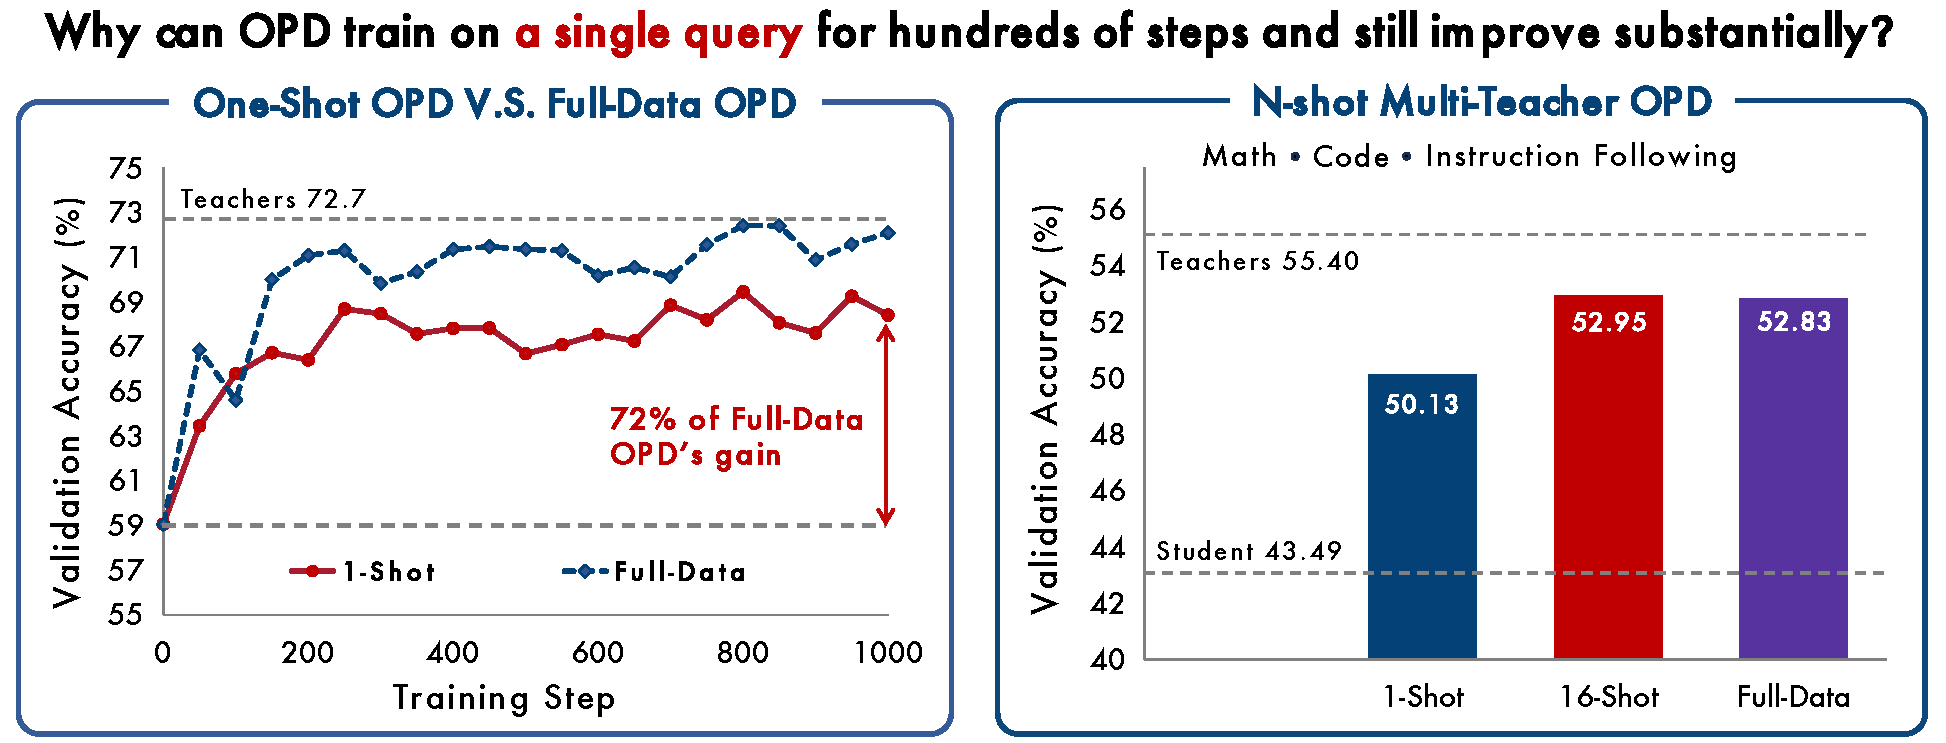
\includegraphics[width=\linewidth]{figures/main1.pdf}
        \captionof{figure}{%
            A single query recovers most of full-data OPD's gain on mathematical reasoning (left), and the effect holds across domains and model families. Under multi-teacher OPD, 16 queries per domain match full-data training (right).
        }
        \label{fig:teaser}
    \end{center}
    \vskip4pt
}

\begin{document}

\maketitle
\newpage


\section{引言}
\label{sec:intro}

同策略蒸馏（OPD）在前沿大模型的后训练中正变得越来越普遍。  
Qwen3~\citep{yang2025qwen3}、MiMo~\citep{xiao2026mimo}、GLM-5~\citep{zeng2026glm}、DeepSeek-V4~\citep{xu2026deepseek} 以及 kimi K3~\citep{team2026kimi} 均结合使用了 OPD、监督微调（SFT）和强化学习（RL）。  
OPD 的独特之处在于其将同策略状态访问与稠密蒸馏监督相结合~\citep{gu2024minillm,agarwal2024policy}。  
学生模型会采样自身的轨迹，而教师模型则在每个访问过的前缀处提供完整的下一个 token 分布，从而生成稠密的、逐 token 的监督信号，而非强化学习中通常使用的单一结果级奖励（具有可验证奖励的强化学习，RLVR）。

越来越多的研究系统地探讨了OPD的训练动态与机制，主要从算法视角出发，解释该方法为何以及如何有效~\citep{li2026rethinking,fu2026revisiting,cai2026learning,zhu2026many}。然而，此前尚无研究探讨过训练数据如何塑造OPD，或数据与算法之间的相互作用。填补这一空白对于全面理解OPD至关重要。在RLVR中，\citet{wang2025oneshot} 引入了一次性RLVR作为一种极端控制实验，以分离出训练数据的作用。我们采用相同的实验视角对OPD进行研究，即仅使用单一查询进行训练，这种情景我们称之为一次性OPD。令我们惊讶的是，一次性OPD产生的学习曲线与一次性RLVR极为相似，如图~\ref{fig:teaser}所示：尽管反复在单一查询上进行训练，模型仍能在数百步内持续提升，并最终取得显著性能增益。因此，本文致力于回答一个核心问题：

\textit{为什么OPD在仅用一个样本训练的情况下，\textbf{能够持续学习如此之久}并且\textbf{取得如此大的提升}？}

\begin{figure}[!ht]
    \centering
    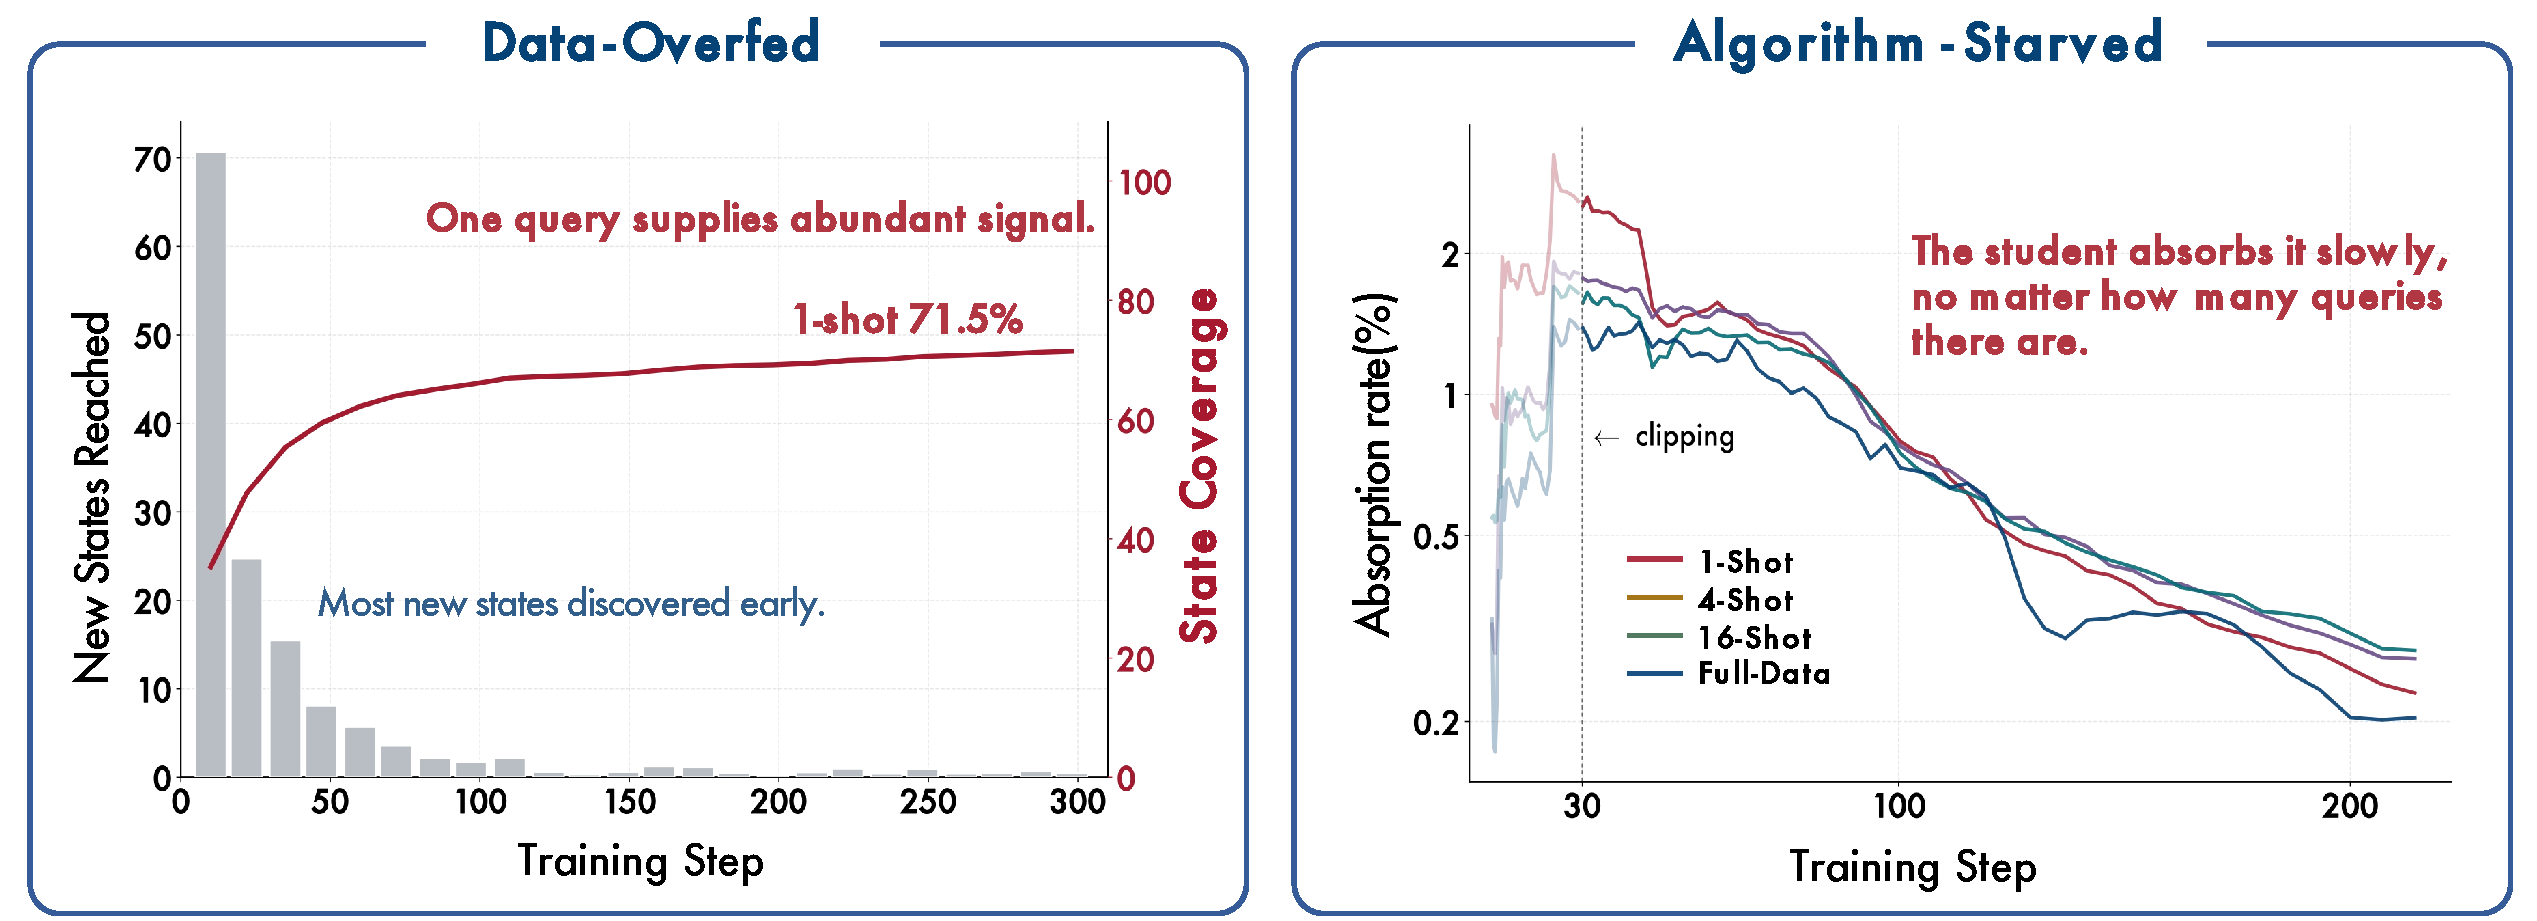
\includegraphics[width=\linewidth]{figures/main2.pdf}
    \caption{\textbf{OPD存在数据过载但算法匮乏的问题。} \textbf{数据：} 一次查询已覆盖大部分全数据OPD访问的状态。 \textbf{算法：} 无论学生模型训练了多少次查询，其吸收剩余教师-学生差距的比例始终越来越小。}
    \label{fig:overview}
\end{figure}

这个问题揭示了同策略教学（OPD）效率的两个方面，而标准训练将它们纠缠在一起：
\textit{\textbf{持续学习如此之久}} 关注的是 \textit{算法} 吸收监督信号的速度，而 \textit{\textbf{提升如此之大}} 则关注为何少量的 \textit{数据} 便足以提供充分的监督。
通过将数据供给缩减至极小点，one-shot OPD 将这两个方面解耦，而这一现象本身表现出很强的鲁棒性：其增益在四个任务领域和三个模型家族中均成立，并且即使在学生从未解决过的查询上依然有效 (\Cref{sec:one-shot})。
我们的答案是：\textbf{OPD 是数据过饱但算法饥饿}。
从 \textit{数据视角} 看，一个查询通过其轨迹所达到的 \emph{状态} 作用于学生，每个状态都是一个前缀 \(s=(x,y_{<i})\) ，在此处教师提供 token 级别的监督，因此一个查询集的价值取决于其所覆盖的状态空间部分。我们通过 \emph{状态覆盖} 来量化这一点：我们将全数据 OPD 所访问的状态分组为语义簇，并报告某一情景下轨迹所达到的比例。单个查询本身已能提供足够的状态，覆盖全数据 OPD 所访问内容的 \(71.5\%\) ，而 16 个语义多样性的查询则覆盖了 \(98.9\%\) 并达到了全数据训练的效果 (\Cref{sec:data})。这就是为何如此少的数据却能极大提升学生表现的原因。从 \textit{算法视角} 看，随着训练进行而下降的是 \emph{吸收率}，即一次更新能够弥补的剩余师生差距比例，其下降趋势在单个查询与全部 17k 查询上几乎相同 (\Cref{sec:algorithm})，因此运行速度是 OPD 本身的特性，而非训练集的属性。
换句话说，单个查询所提供的监督在很大程度上未被充分利用，其利用速率受限于同策略学生吸收信息的速度。

相同的机制同样适用于超越 one-shot 情景的数据设计。在多教师 OPD（MOPD）~\citep{xiao2026mimo,xu2026deepseek} 中，单个学生在多个领域上进行训练，每个查询被路由到其对应领域的教师，我们发现每个领域只需 16 个语义多样性的查询即可达到全数据训练的效果 (\Cref{sec:mopd})。将数据设计推向极致，我们进一步表明，即使一个不描述任何问题的训练输入仍可保持有效性：跨领域 WildChat 提示和无内容模板对 OPD 的驱动效果几乎与完整训练集相当 (\Cref{sec:template})。因此，输入之所以有效，主要在于它能够启动学生的推理过程。此外，我们在相同查询上对 one-shot RLVR 进行了受控对比，以明确算法差异：在几乎每次滚动中，一旦查询被解决，RLVR 的奖励即被耗尽；而 OPD 的 token 级信号在整个训练过程中持续存在，且 OPD 在 $1000$ 步内的验证增益超过 RLVR 的两倍 (\Cref{sec:opd-vs-rlvr})。

简而言之，OPD 所获得的监督信息超出了其算法所能吸收的范围。因此，数据监管需要解决的问题不再是收集多少问题，而是输入所引发的状态是什么。我们希望这种对训练数据的状态层面的理解，能为未来通过所引发的状态来选择查询，以及提高学生吸收这些信息的速率提供指导。

\section{初步研究}
\label{sec:prelim}

\subsection{符号标记}
令 $x\sim\mathcal{D}$ 表示一个 \emph{训练输入}，$y=(y_1,\ldots,y_L)$ 表示一个响应，其中 $y_{<i}=(y_1,\ldots,y_{i-1})$ 是到 token 位置~$i$ 为止的前缀。我们考虑两个大模型：一个学生 $\pi_{\theta}$ 和一个教师 $\pi_T$ ，每个模型在共享词表上定义一个下一个 token 分布。一个 \emph{轨迹} 是一对 $(x,y)$ ，其中 $y$ 从给定 $x$ 的策略中自回归采样得到。我们使用 $i$ 来索引 token 位置，$t$ 来索引最优化步骤，用 $\theta_t$ 表示第~$t$ 步时的学生参数。一个 \emph{状态} 是自回归上下文 $s_i=(x,y_{<i})$ ，即 OPD 目标所定义的对象。 

\subsection{同策略蒸馏}
同策略蒸馏（OPD）从学生模型采样轨迹，并将学生模型在实际访问的前缀上对齐到教师模型~\citep{agarwal2024policy}。OPD也可视为一种稠密KL约束强化学习的特例，其中教师分布诱导出一个token级别的奖励，且KL正则化项具有固定的相对权重~\citep{yang2026learning}。

在全分布形式中，OPD 在访问的状态上最小化每个 token 的 KL 散度：
\begin{equation}
    \mathcal{L}_{\mathrm{OPD}}(\theta)
    =
    \mathbb{E}_{x\sim\mathcal{D},\,y\sim\pi_\theta}
    \left[
        \sum_{i=1}^{L}
        \operatorname{KL}\!\left(
            \pi_\theta(\cdot\mid s_i)
            \,\Vert\,
            \pi_T(\cdot\mid s_i)
        \right)
    \right].
\end{equation}

实际上，我们用每个 token 的优势来估算它：
\begin{equation}
    A_i^{\mathrm{OPD}} = \log \pi_T(y_i \mid s) - \log \pi_\theta(y_i \mid s),
    \label{eq:token-advantage}
\end{equation}

其中 $s = (x, y_{<i})$。由此公式可得出两个性质：(i) 该信号是\emph{局部}的，即仅依赖于状态~$s$ 处的预测问题，而不依赖于轨迹的结果；(ii) 该信号是\emph{稠密}的，即教师在每个访问过的状态处提供分布信号，而非仅在终端提供标量奖励。

公式~\ref{eq:token-advantage} 仅在学生输出的 token 上评估修正。对同一散度的第二个估计量在每个访问的状态下保留学生最可能的 $k$ 个 token，并按学生的概率对其进行加权：
\begin{equation}
    A_i^{\text{top-}k}
    =
    \sum_{v \in \mathcal{V}_i}
    \tilde{\pi}_\theta(v \mid s)
    \left[
        \log \pi_T(v \mid s) - \log \pi_\theta(v \mid s)
    \right],
    \label{eq:topk-advantage}
\end{equation}
其中，$\mathcal{V}_i = \operatorname{TopK}(\pi_\theta(\cdot \mid s), k)$ 和 $\tilde{\pi}_\theta$ 是在该集合上 $\pi_\theta$ 规范化的结果。它将散度截断为 $k$ 项，而非通过一个样本 token 进行估计，以分布的尾部为代价换取更低的方差。第~\ref{sec:setup} 节说明了每次运行所使用的具体形式。以下的对齐度量是根据两个策略记录的分布计算出的诊断指标，因此在任一形式下均可获得。



\subsection{动态指标}

\paragraph{间隙恢复。}
由于评估标准和初始师生模型性能差距在不同领域和模型对之间存在差异，原始得分提升无法直接比较。因此，我们报告提升幅度相对于初始师生差距的比率。令 $M_0$、$M_T$ 和 $M_t$ 分别表示初始学生模型、教师模型以及优化步骤~$t$ 时的学生模型的评估得分。在步骤~$t$ 的差距恢复比率为
$\frac{M_t-M_0}{M_T-M_0}\times100\%.$ 
当该值为 $0\%$、$100\%$ 或高于 $100\%$ 时，分别表示未向教师模型靠拢、与教师模型持平或超越教师模型。

\paragraph{完整数据恢复。}
当参考对象为全数据 OPD 而非教师模型时，我们改用全数据 OPD 的增益进行归一化。令 $M_F$ 表示在同一最优化步骤下的全数据 OPD 得分。全数据恢复比为
$\frac{M_t-M_0}{M_F-M_0}\times100\%.$  当该值接近 $100\%$ 时表示减少的查询集几乎达到了全数据 OPD 的增益，而当该值高于 $100\%$ 时则表示其超过了全数据 OPD 的增益。


\paragraph{Top-$k$  token 重叠率。}
该指标衡量两个策略的高概率 token 集合之间的一致性。令 $S_t^\theta(s)=\operatorname{TopK}(\pi_{\theta_t}(\cdot\mid s),k)$  和 $S^T(s)=\operatorname{TopK}(\pi_T(\cdot\mid s),k)$ 。在最优化步骤~$t$ 时的重叠为
\begin{equation}
    O_t^{(k)}
    =
    \frac{1}{|\mathcal{T}_t|}
    \sum_{i\in\mathcal{T}_t}
    \frac{|S_t^\theta(s_i)\cap S^T(s_i)|}{k},
    \label{eq:topk-overlap}
\end{equation}
其中，$\mathcal{T}_t$ 索引了在步骤~$t$ ~\citep{li2026rethinking} 收集的批量滚动数据中非填充的响应位置。

\paragraph{重叠token优势。}
在该协议中，我们对教师-学生对数概率差异在共享 token $S_t^\theta(s_i)\cap S^T(s_i)$ 上进行平均，并根据学生对该 token 的概率赋予每个共享 token 以权重。该结果反映了在两个策略均已给予较高秩的 token 上，二者政策之间的距离。由于这种加权方式，以及它是在 top-$k$ 项上而非采样 token 上进行平均，因此其量级远小于第~\ref{sec:rate-setup} 节中的教师-学生距离，两者的数值水平不可直接比较。

\section{一次成像现象}
\label{sec:one-shot}

本节介绍了 One-Shot OPD 的实验设置与结果。我们研究了 \textit{single query 能够恢复 full-data OPD 的多少收益，以及该收益的鲁棒性如何}。

\begin{tcolorbox}[takeawaysbox]
\textbf{一次查询即可引发稳健的OPD收益。}
单次查询即可在任务领域和模型族之间恢复大部分教师-学生差距。该收益对查询难度、响应长度和采样温度均不敏感，即使学生从未解决过的查询，其效果也与总是能解决的查询相当。
\end{tcolorbox}

\subsection{实验设置}
\label{sec:setup}

我们建立了一次性OPD，涵盖数学、代码生成、指令遵循和智能体工具使用，以进行受控分析，测试其通用性。

\paragraph{模型}

\begin{table}[t]
\centering
\small
\caption{
实验中使用的师生配对。
}
\label{tab:full}
\setlength{\tabcolsep}{5pt}
\renewcommand{\arraystretch}{1.12}
\begin{tabularx}{\textwidth}{@{}lXX@{}}
\toprule
\textbf{Setting} & \textbf{Student} & \textbf{Teacher} \\
\midrule

\multirow{3}{*}{Mathematical reasoning}
& DeepSeek-R1-Distill-Qwen-1.5B\newline
{\footnotesize (R1-Distill-1.5B)}
& JustRL-DeepSeek-1.5B\newline
{\footnotesize (JustRL-1.5B)} \\

& Llama-3.2-3B-Instruct\newline
{\footnotesize (Llama-3B-It)}
& GT-Llama-3.2-3B-Instruct-MATH\newline
{\footnotesize (GT-Llama-3B-Math)} \\

& OLMo-3-7B-Instruct-DPO\newline
{\footnotesize (OLMo-7B-It-DPO)}
& OLMo-3-7B-Instruct\newline
{\footnotesize (OLMo-7B-It)} \\

\midrule

Code generation
& DeepSeek-R1-Distill-Qwen-1.5B\newline
{\footnotesize (R1-Distill-1.5B)}
& Nemotron-Research-Reasoning-Qwen-1.5B-v2-RLVE\newline
{\footnotesize (Nemotron-1.5B)} \\

Instruction following
& DeepSeek-R1-Distill-Qwen-1.5B\newline
{\footnotesize (R1-Distill-1.5B)}
& UltraData-IF-1.5B \\

Agentic tool use
& Qwen2.5-Coder-1.5B-Instruct\newline
{\footnotesize (Qwen-Coder-1.5B)}
& Hammer2.1-1.5b\newline
{\footnotesize (Hammer-1.5B)} \\

\bottomrule
\end{tabularx}
\end{table}

对于每个领域，我们将一个学生模型与同家族的微调后教师模型配对。表~\ref{tab:full} 列出了完整的标识符以及全文中使用的简称。数学、代码生成和指令遵循任务共享同一个学生模型 R1-Distill-1.5B \citep{deepseekai2025deepseekr1incentivizingreasoningcapability}，其对应的教师模型分别为 JustRL-1.5B \citep{he2025justrl}、Nemotron-1.5B \citep{zeng2025rlve}，以及我们从同一学生模型微调得到的一个指令遵循变体（见附录~\ref{app:IF-setup}）。在 Agentic 工具使用场景中，学生模型为 Qwen-Coder-1.5B \citep{hui2024qwen2}，教师模型为 Hammer-1.5B \citep{lin2024hammer}。为了检验该现象是否仅针对基于 Qwen 的模型对，我们还引入了来自其他家族的两个数学推理模型对：Llama-3B-It \citep{grattafiori2024llama} 与 GT-Llama-3B-Math \citep{zhang2025co}，以及 OLMo-7B-It-DPO 与 OLMo-7B-It \citep{olmo2025olmo}。

\paragraph{数据集}
领域特定的训练集包括用于数学推理的DAPO-Math-17K \citep{yu2026dapo}、用于代码生成的Open-R1 Codeforces \citep{penedo2025codeforces}、用于指令遵循的UltraData-SFT-2605 \citep{ultradata-sft-2605}的采样子集，以及用于智能体工具调用的xLAM-function-calling-60K \citep{liu2024apigen}。对于数学领域的one-shot OPD，我们选取了三个查询，覆盖简单、中等和困难三种初始难度，其得分基于学生在训练前8次滚动测试中的通过率（分别对应\(8/8\)、\(4/8\)和\(0/8\)）。在其他领域中，one-shot查询则从相应训练集中随机采样。附录~\ref{app:model-data}详细介绍了数据集预处理过程及所选的one-shot查询。

\paragraph{训练}
我们在 \texttt{veRL} \citep{sheng2025hybridflow} 中实现了 OPD。  
本节的数学推理运行优化公式~\ref{eq:topk-advantage} 的前-\(k\) 优势，使用 \(k=16\)；代码、指令遵循和 Agentic 运行则优化公式~\ref{eq:token-advantage} 的采样 token 优势。  
每次更新均使用 $64$ 次 rollout 构成的批量。我们采用 AdamW 优化器，学习率为 $10^{-6}$，rollout 温度为 $1.0$，梯度裁剪范数为 $1.0$；其余超参数列于表~\ref{tab:opd-hyperparams} 中。


\paragraph{评估。}
对于数学任务，我们在 MATH-500 \citep{hendrycksmath2021}、AMC 2023 \citep{li2024numinamath} 和 AIME 2025 \citep{balunovic2026matharena} 上进行评估，每个问题采样 16 个响应，并报告 avg@16 准确率。  
对于代码生成任务，LiveCodeBench v6 (LCB v6) \citep{jain2025livecodebench} 每个问题使用 3 个采样解法，并通过官方基于执行的评估器报告 avg@3 得分。  
对于指令遵循任务，Multi-IF \citep{he2024multi} 评估三轮对话，并报告其八种语言上最终一轮的平均得分。  
对于 Agentic 工具使用任务，BFCL v3 \citep{patil2025bfcl} 报告所评估子集上的 avg@8 得分。响应长度上限分别为：\(31{,}744\) token 用于数学任务，\(65{,}536\) token 用于 LCB v6，\(16{,}384\) token 每轮用于 Multi-IF，以及 \(4{,}096\) token 用于 BFCL v3。除非另有说明，数学任务的结果报告的是在 MATH-500、AMC 2023 和 AIME 2025 上验证准确率的宏平均值，虚线标记教师模型表现。


\begin{figure}[t]
  \centering
  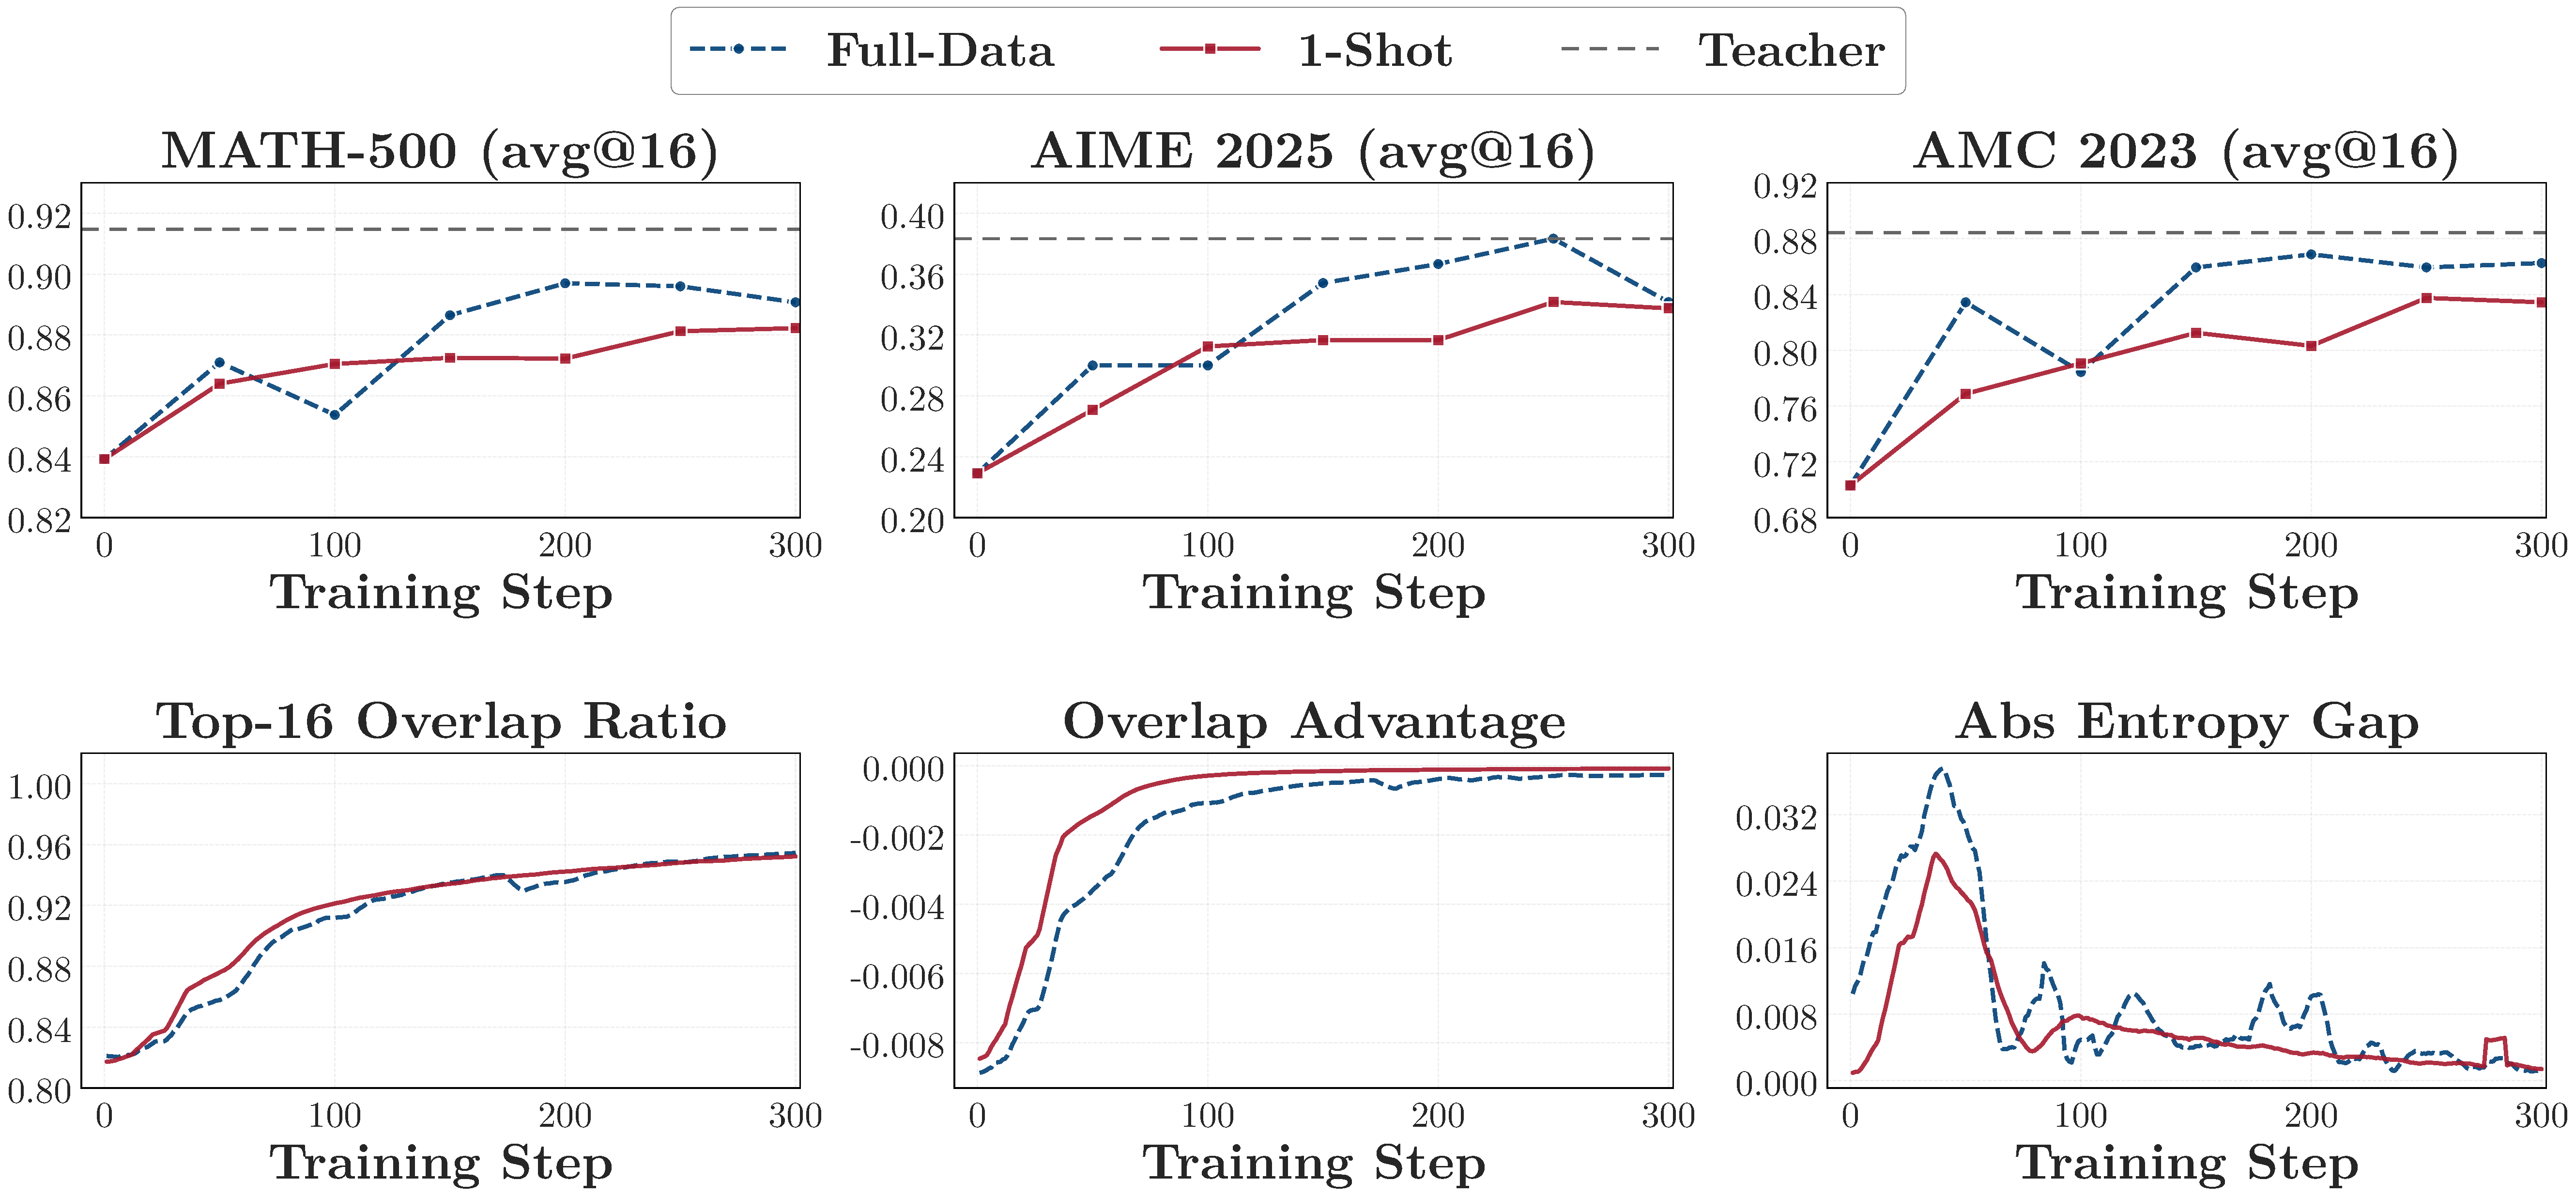
\includegraphics[width=\textwidth]{figures/3_oneshot_math300.pdf}
  \caption{one-shot OPD 在数学推理上的验证准确率和训练动态。}
  \label{fig:math_oneshot_dynamics}
\end{figure}

\begin{figure}[t]
  \centering
  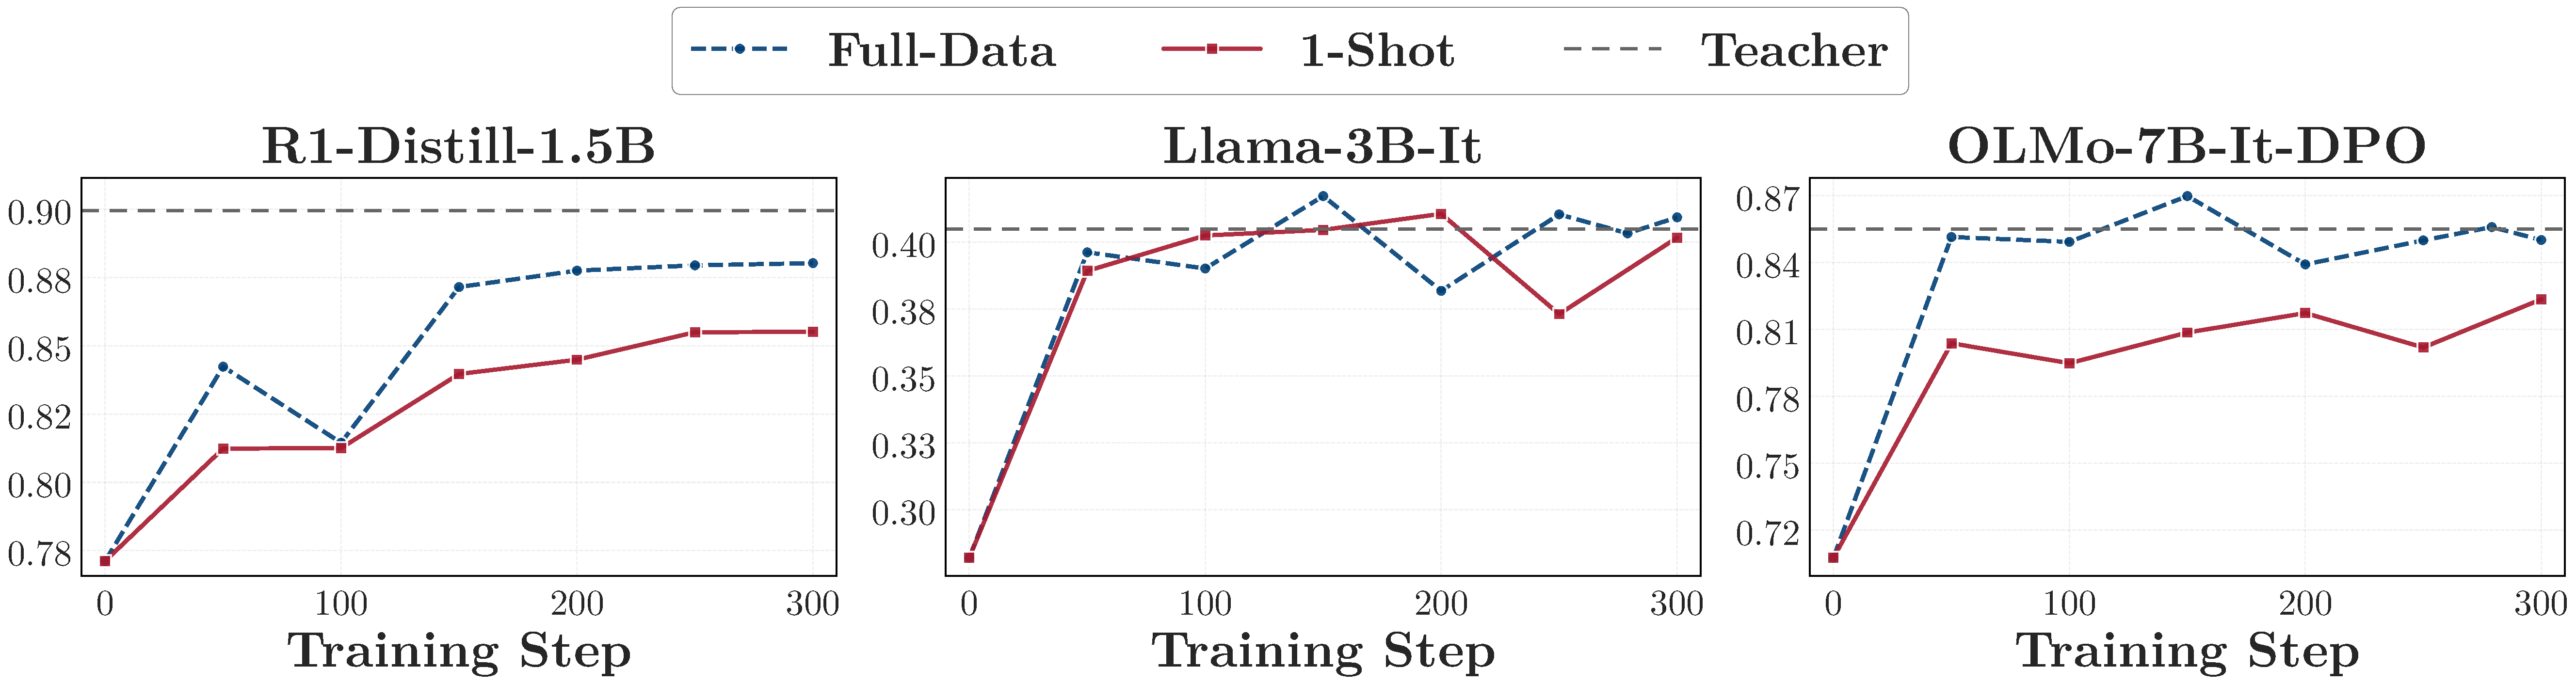
\includegraphics[width=\textwidth]{figures/3_cross_family.pdf}
  \caption{
  在数学推理任务上，对三个学生-教师模型族进行one-shot OPD的验证准确率，结果为MATH-500和AMC 2023的平均值。由于Llama模型对AIME 2025的得分接近零，因此该数据集被排除。
  }
  \label{fig:cross_family}
\end{figure}

\begin{figure}[t]
  \centering
  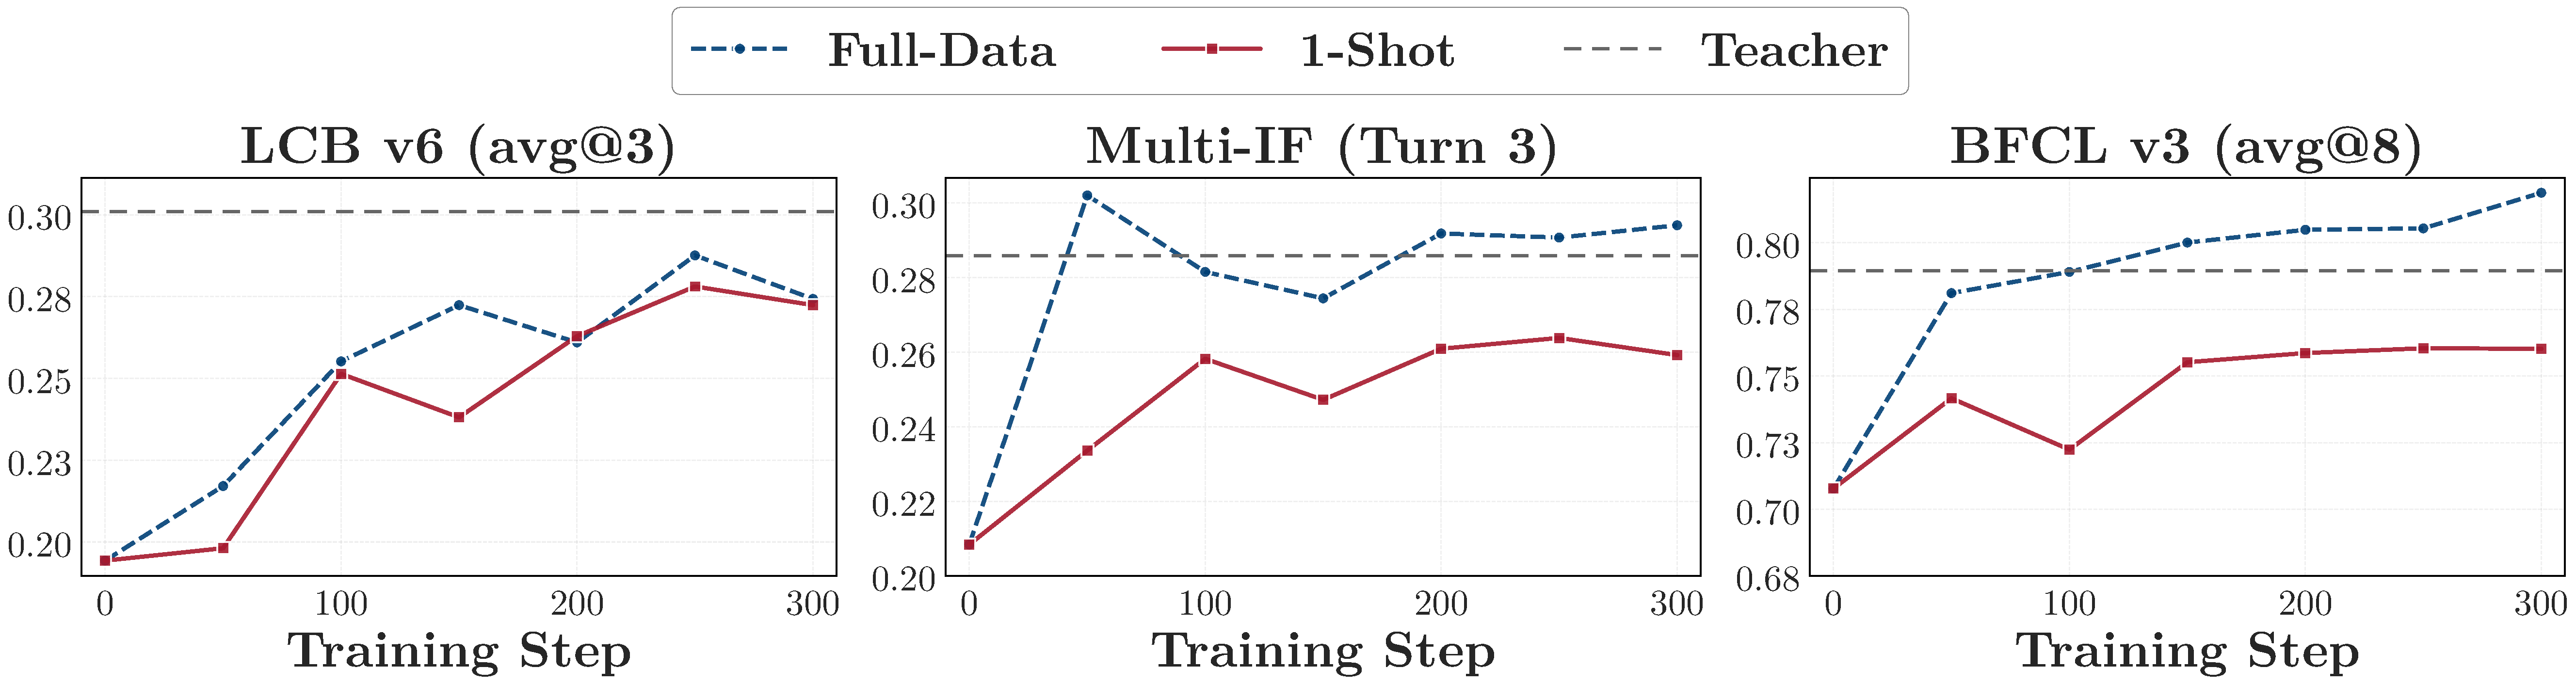
\includegraphics[width=\textwidth]{figures/3_cross_domain.pdf}
  \caption{
  one-shot OPD 在三个任务领域中的验证准确率。
  }
  \label{fig:cross_domain}
\end{figure}

\begin{figure}[t]
  \centering
  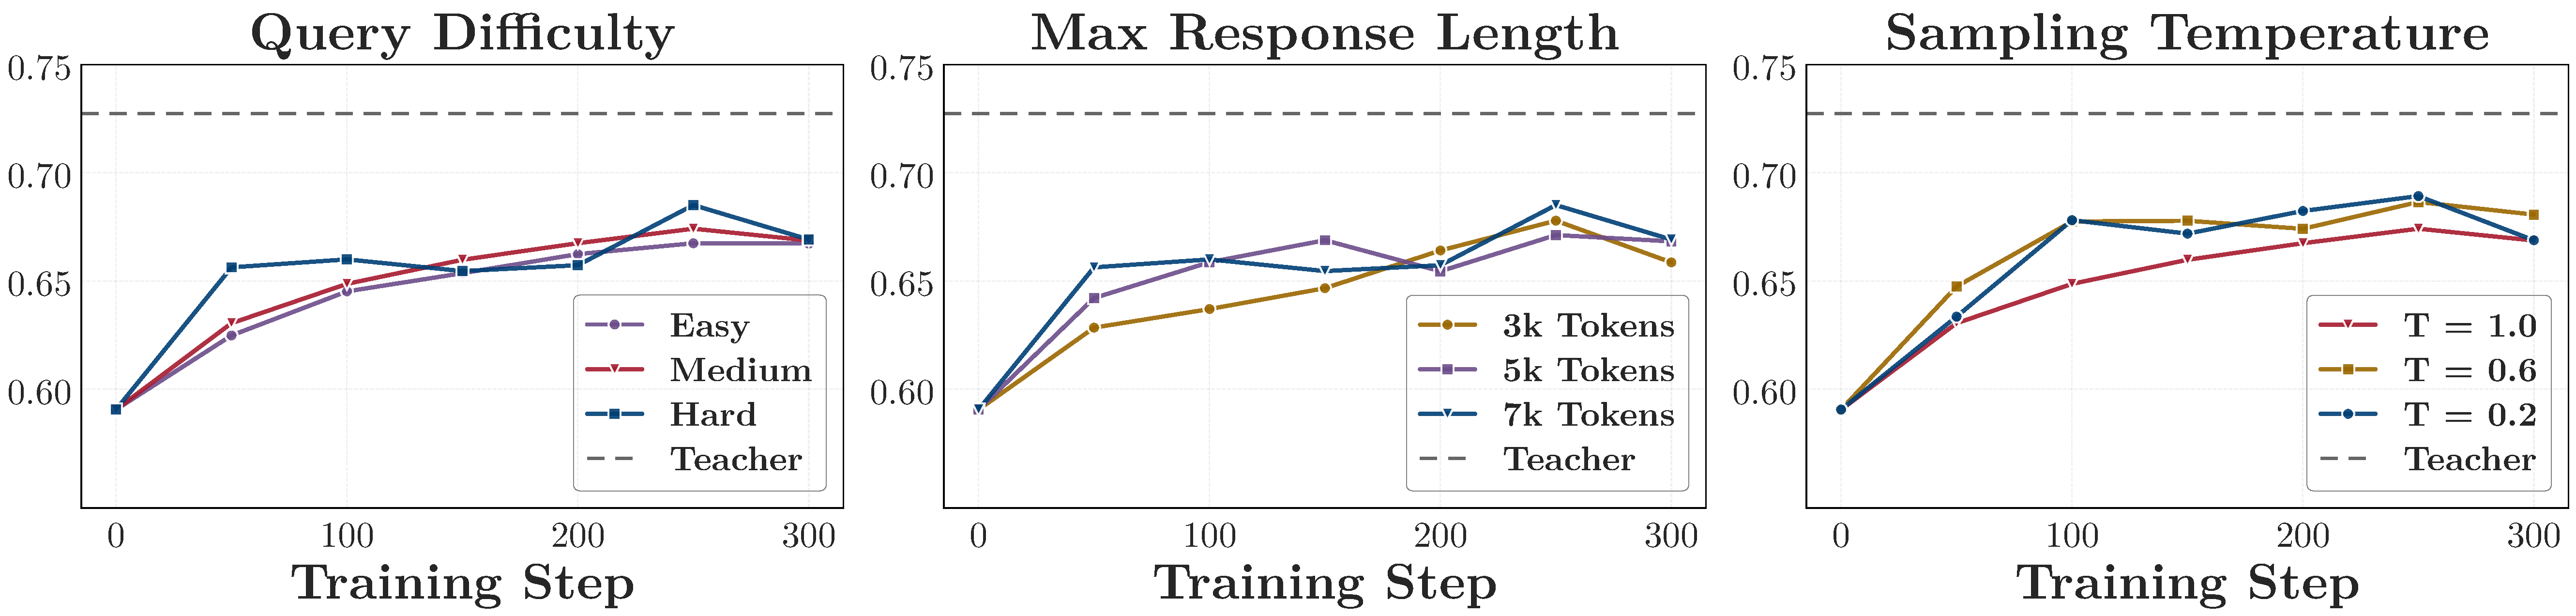
\includegraphics[width=\textwidth]{figures/3_ablations.pdf}
  \caption{
  在不同查询难度、硬查询的响应长度限制以及中等查询的采样温度下，one-shot OPD 的验证准确率。
  }
  \label{fig:probe_prompt}
\end{figure}


\subsection{实验结果}
\label{sec:finding-recovery}

\paragraph{One-shot OPD 在数学上恢复了大部分全数据 OPD 的增益。}

图~\ref{fig:math_oneshot_dynamics} 表明，在单个查询上进行训练可提升在 MATH-500、AIME 2025 和 AMC 2023 上的准确率，使其在所有三个基准上均接近全数据 OPD。三者平均来看，one-shot OPD 达到 \(68.5\) ，而全数据 OPD 为 \(69.8\) ，恢复了教师-学生差距的 \(69\%\) ，以及全数据 OPD 在第 300 步时增益的 \(87\%\) 。超过第 \(300\) 步后，两条曲线始终维持在约 \(3\) 个点的范围内，恢复比例从 \(62\%\) 到 \(89\%\) ，持续至第 \(1000\) 步，此时 one-shot OPD 达到 \(68.4\) 对比 \(72.1\) ，恢复了全数据 OPD 增益的 \(72\%\) （图~\ref{fig:teaser}）。在两种情景下，训练动态遵循相同的对齐过程：top-16 重叠率上升至全数据水平，重叠 token 优势趋近于零，绝对熵差几乎完全闭合。因此，即使所有回溯轨迹均源自单一查询，OPD 仍能提升准确率，并逐步将学生分布与教师在访问状态上的分布对齐。


\paragraph{one-shot效应在不同家族和任务领域中均具有鲁棒性。}
\label{sec:one-shot-robust}
图~\ref{fig:cross_family} 表明，one-shot OPD 在所有三个学生-教师模型族中均提升了数学推理能力。在最终检查点，平均得分分别从对应的学生基准的 \(77.1\) 、\(28.2\) 和 \(70.8\) 提升至 R1-Distill-1.5B、Llama-3B-It 和 OLMo-7B-It-DPO 的 \(85.5\) 、\(40.2\) 和 \(82.4\) 。图~\ref{fig:cross_domain} 进一步表明，该效果不仅限于数学推理：在代码生成、指令遵循和 Agentic 工具使用任务上，one-shot OPD 分别恢复了 \(73\%\) 、\(66\%\) 和 \(64\%\) 的相应教师-学生差距。综上所述，这些结果表明，one-shot 效应在模型族和任务领域之间均具有鲁棒性。


\paragraph{one-shot 效应对于查询和展开特性具有鲁棒性。}

我们接下来考察在不同查询难度、响应长度预算以及轨迹采样温度下，one-shot OPD 是否依然有效。如图~\ref{fig:probe_prompt} 所示，无论查询是简单、中等还是困难，one-shot OPD 均能发挥作用，尽管三种情景下正确轨迹的比例演化方式差异显著（附录~\ref{app:training-accuracy}）：简单查询几乎每一步都能解决，中等查询在训练过程中逐渐变得可解，而困难查询始终无法解决。收紧响应长度上限和降低轨迹采样温度均能保持 one-shot 的优势。综合来看，这些结果表明，one-shot OPD 对查询难度、响应长度预算以及轨迹采样温度具有鲁棒性。

\section{数据视角：丰富状态}
\label{sec:data}

第~\ref{sec:one-shot}节表明，One-Shot OPD 稳健地恢复了全数据 OPD 的大部分增益。本节提出问题：\textit{为什么对单个查询进行训练会产生如此大的增益，以及同样的解释是否也涵盖了 n-shot OPD 能够匹配全数据 OPD 的情况}。 \footnote{此处分析的运行以及第~\ref{sec:algorithm} 节中的运行优化的是公式~\ref{eq:token-advantage} 中的采样 token 优势，而不是第~\ref{sec:one-shot} 节数学运行中使用的前 \(k\) 个 token 优势，因此它们的绝对准确率与该处报告的结果略有不同。下面的每一项比较都是在具有此形式的运行之间进行的。}

\begin{tcolorbox}[takeawaysbox]
\begin{itemize}[topsep=0pt, partopsep=0pt, leftmargin=12pt, itemsep=0pt]
    \item  \textbf{一次查询已经覆盖了大部分全数据状态空间。}
OPD 主要消耗的是状态而非查询。在实际应用中，从单个查询重复展开可以在 \(71.5\%\)  步内达到 \(100\)  的状态覆盖，其中大部分覆盖发生在前 \(100\)  步内。

    \item  \textbf{尽管查询种类多样，但仅有少数查询能达到充分状态，并逼近全数据性能。} 增加语义上不同的查询能够同时提升状态覆盖和验证准确率，16个查询已达到全数据OPD水平。一个额外样本的价值在于其是否覆盖了先前样本未涉及的状态。
\end{itemize}
\end{tcolorbox}

\subsection{one-shot OPD 的状态覆盖}
\label{sec:state-coverage}

\paragraph{设置}
OPD 在状态上进行训练，而非在查询上。一个查询 \(x\) 与一个采样得到的响应 \(y\) 会在每个 token 位置 \(i\) 生成一个状态 \(s=(x,y_{<i})\) ，每个状态都与来自教师模型的目标分布配对。每次更新有 \(64\)  次滚动，即使单个查询也能产生数万个监督状态，因此查询数量可能会严重低估 OPD 所能获得的监督量。

\begin{tcolorbox}[examplebox, title={Hypothesis}]
单个查询若能覆盖全数据OPD所访问状态空间的广泛区域，则可提供足够的监督信息，以恢复大部分全数据OPD的收益。
\end{tcolorbox}

为了验证这一假设，我们测量的是访问状态的广度而非访问状态的总数，因为每个生成的 token 都会产生一个独特的前缀。我们称此度量为 \emph{状态覆盖}：我们将状态表示在共享的表示空间中，将该空间划分为簇，并报告某一情景的采样路径所达到的比例。
\begin{itemize}[topsep=1pt, partopsep=0pt, leftmargin=13pt, itemsep=2pt, parsep=0pt]
    \item  \textbf{表示.} 我们通过每个状态的\emph{教师签名} \(h_T(s)\) 来表示，即教师在该状态最后一个token处的最终层隐藏向量。
    \item  \textbf{参考空间。} 我们将全数据 OPD 在 DAPO-Math-17K 上整个运行过程中访问的状态进行汇总，从每次轨迹中均匀采样 \(8\) 个位置。这些轨迹中保留的一部分不参与簇的定义，而是作为独立的情景进行衡量，\emph{全数据（保留）}。\footnote{每五个收集到的样本中有三个构成训练池，其余两个为保留样本，因此它代表了在相同预算下全数据OPD在新样本上所能达到的效果。}
    \item  \textbf{簇。} 经过PAC后，\(K\)-均值将参考特征划分为 \(K=200\) 个簇。每个状态归属于最近的簇，记为 \(c(s)\) 。
\end{itemize}
一个状态集 \(S\)  的 \emph{状态覆盖} 是其达到的 \(K\)  簇的比例：
\begin{equation}
    \mathrm{Cov}(S)
    =
    \frac{1}{K}
    \left|
    \left\{\,c(s)\;:\;s\in S\,\right\}
    \right|.
    \label{eq:state-coverage}
\end{equation}
覆盖记录了某种情景达到的簇，而非访问它们的频率。我们仅对簇进行一次拟合，并在相同的 \(300\) 步数上测量每个情景。全数据（保留测试）在此预算下可达到 \(100\%\) ，因此量表顶端是全数据 OPD 所能达到的水平，而非构造保证的最大值。附录~\ref{app:state-coverage} 给出了构造和调度方案，并表明以下比较在 \(K\) 、参考集和状态位置的不同选择下均保持稳定。

\paragraph{one-shot OPD 达到了状态空间的 \(71.5\%\)。}
\begin{figure}[t]
  \centering
  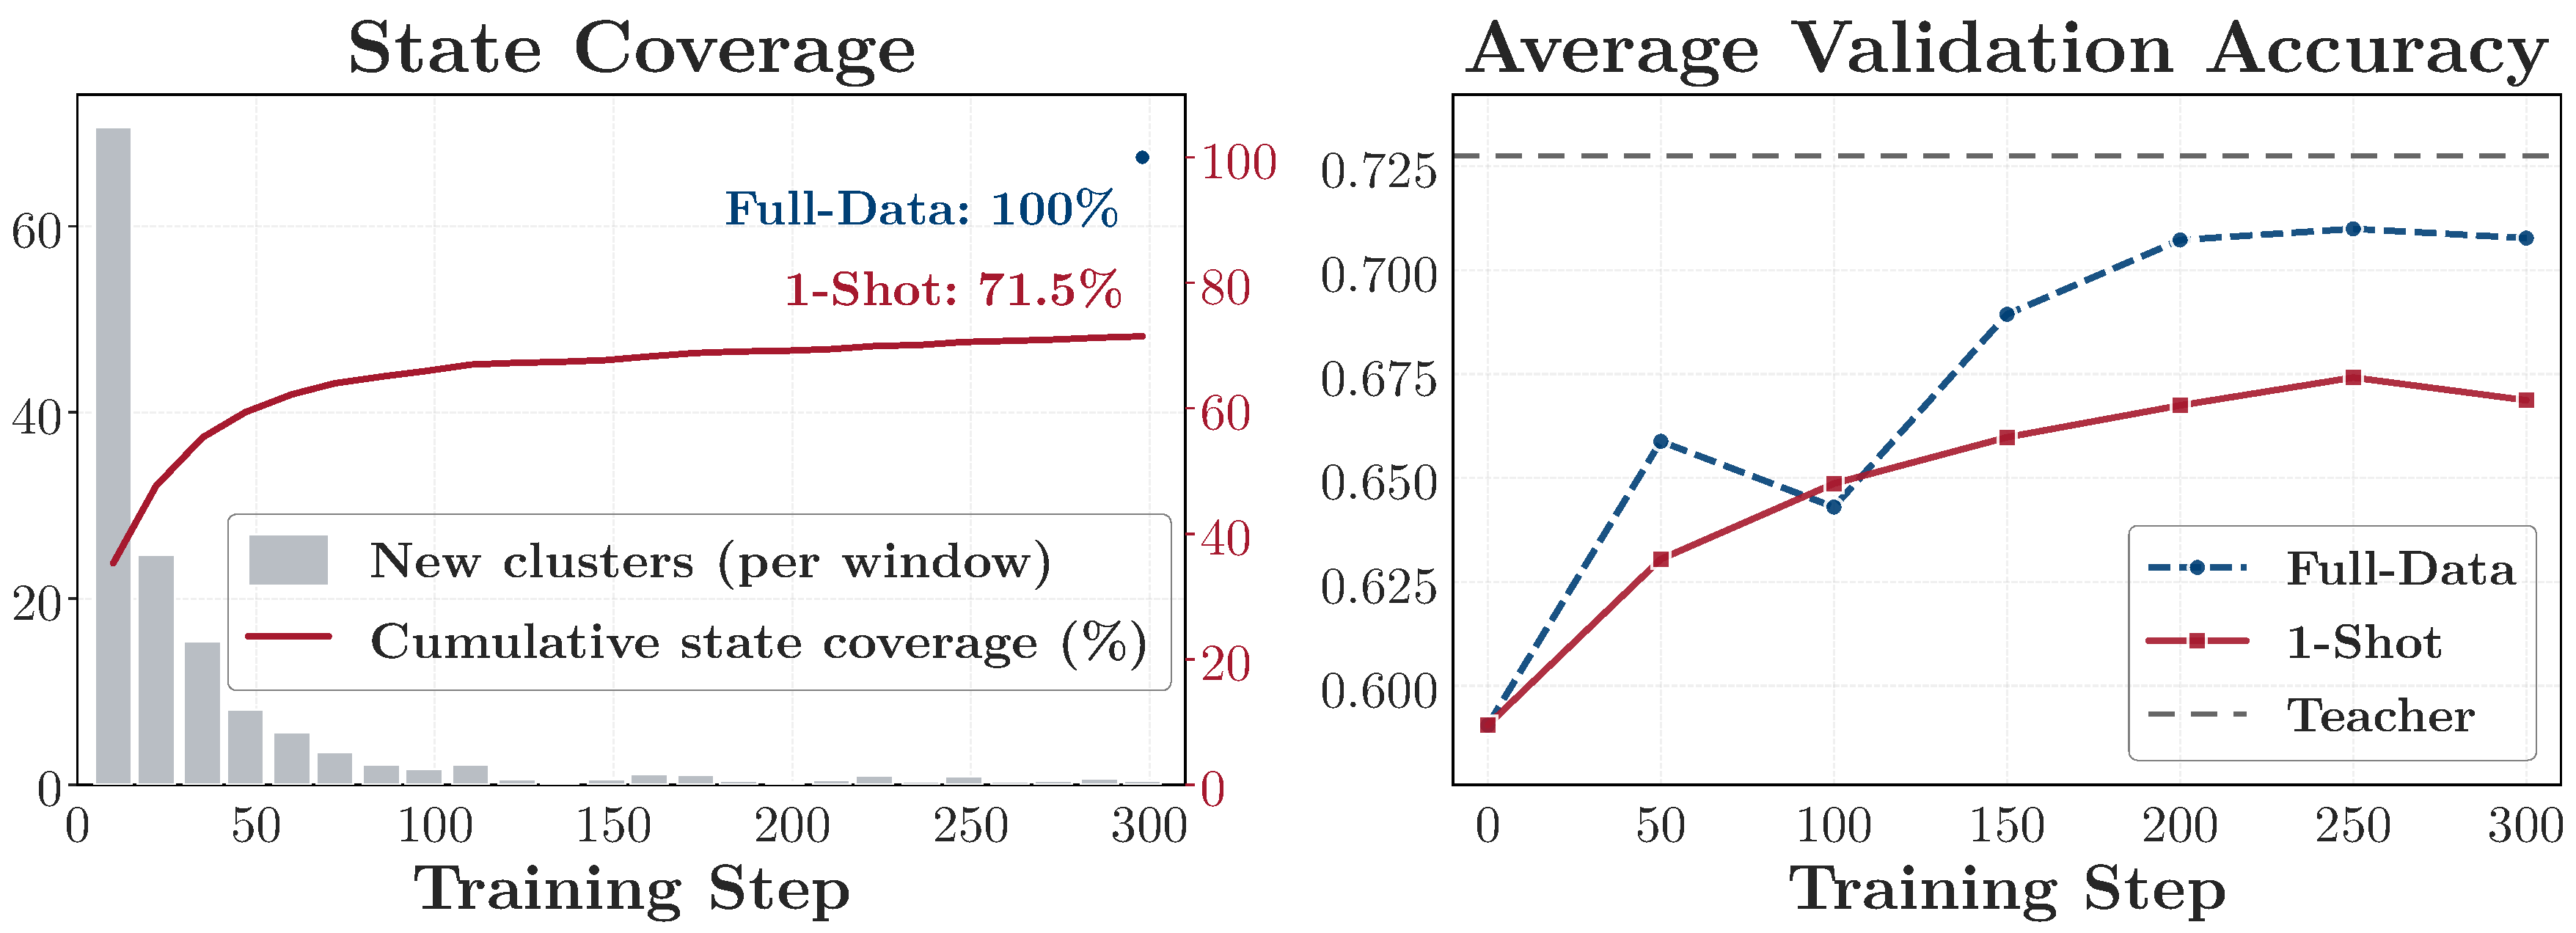
\includegraphics[width=0.75\linewidth]{figures/4_state_coverage_oneshot.pdf}
  \caption{
    one-shot OPD 在中等查询下的状态覆盖与验证准确率，与全数据 OPD 进行对比。覆盖度是相对于全数据 OPD 所能达到的状态空间进行衡量的，因此其水平为 \(1.0\) ，而非分离的曲线。
  }
  \label{fig:state-coverage}
\end{figure}
图~\ref{fig:state-coverage} 显示，one-shot OPD 在步骤 \(300\) 时达到 \(71.5\%\) 状态覆盖。其中大部分覆盖在早期就已出现：该运行在步骤 \(100\) 时达到 \(65.9\%\)，随后在接下来的 \(200\) 步中仅增加了 \(5.6\) 个百分点的覆盖。因此，从同一查询重复展开仍能发现新的簇，但速度显著下降。  
同一运行将验证准确率从 \(59.1\) 提升至 \(66.9\)，而 full-data OPD 在步骤 \(300\) 时仅为 \(70.8\)。这些结果在数据方面也呈现出相同的模式：单次查询已覆盖 full-data OPD 所能达到的大部分状态空间簇，并带来显著的验证性能提升。因此，one-shot OPD 查询次数较少，却能生成广泛的有效监督。

\subsection{多样性扩展状态覆盖}
\label{sec:state-diversity}

上述分析表明，一次查询已能覆盖大部分全数据状态空间，但因果问题仍待澄清：训练表现良好的运行可能只是沿途访问了更多状态，而这些额外状态并未实际发挥作用。因此，我们直接消融状态覆盖，固定其他设置不变，改变训练数据所能达到的不同状态的数量。

\paragraph{设置}
我们从两个方向提升数据多样性，每个方向都有独立的控制机制。
\textbf{(i) 响应多样性（异策略）。} 我们在 one-shot 查询时仅从初始学生中采样一次 \(64\) 轨迹，并保持该样本池固定，从而消除同策略训练中的干扰因素——在同策略训练中，随着学生不断更新，状态会持续变化。嵌套子集保留 \(1\) 、\(4\) 、\(16\) 或全部 \(64\) 条轨迹，并将保留的轨迹重复填充至每个批量大小为 \(64\) 的批次中。所有条件共享相同的查询、批量大小和最优化预算，因此唯一变化的量是不同轨迹的数量，进而影响状态数量。
\textbf{(ii) 查询多样性（同策略）。} 这些实验则改变查询集，且均遵循数学配置。从 one-shot OPD 使用的中等规模查询开始，我们通过使用 BGE-M3~\citep{chen2024bge} 对 DAPO-Math-17K 进行聚类，每种语义簇选取一个代表性查询，构建出 4- 和 16- shot 查询集，确保每次添加到阶梯中的查询与已有查询在语义上均不重复，随后将这些查询集与全数据 OPD 进行对比。
我们报告每次运行的验证准确率，对于同策略运行还报告状态覆盖情况，其中滚动回放指学生在训练过程中实际生成的轨迹。异策略得分在从步骤 \(300\) 到 \(500\) 的五个评估检查点上取平均。在覆盖方面，全数据条形图代表预留的测试集，设定 \(100\%\) 的上限。

\begin{figure}[t]
  \centering
  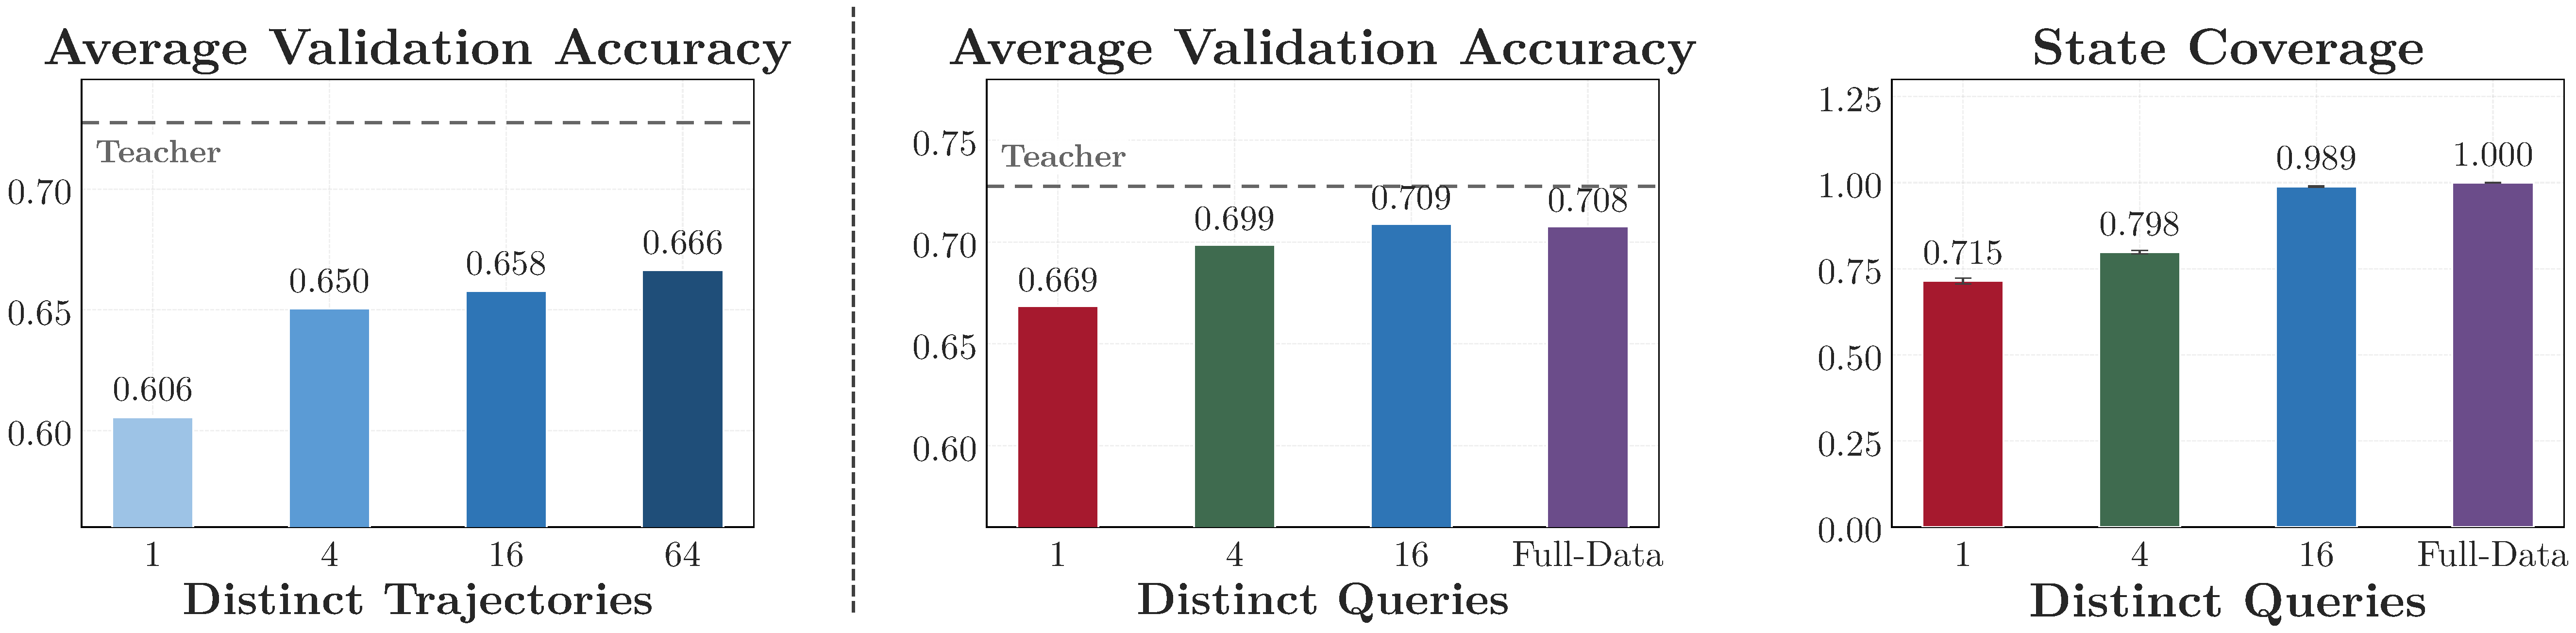
\includegraphics[width=\linewidth]{figures/4_state_diversity.pdf}
    \caption{
    随着训练数据的多样化，验证准确率和状态覆盖情况在响应端通过在不同轨迹上的异策略训练，在查询端通过在不同查询上的同策略训练得到提升。}
  \label{fig:state-diversity}
\end{figure}

\paragraph{数据多样性即状态多样性，少数查询能匹配全数据OPD。}
图~\ref{fig:state-diversity} 显示，随着不同轨迹数量的增加，异策略验证准确率单调上升。其他条件保持不变，因此额外轨迹带来的唯一变化是状态的增加。同策略实验从查询角度得出了相同的结论。语义上不同的查询使验证准确率提升，直到16个查询达到全数据OPD的水平，此时在状态覆盖方面也达到了相同水平，状态覆盖从一个查询时的 \(71.5\%\) 上升至16个查询时的 \(98.9\%\)。梯子上的每一个查询都代表一个新的语义簇，因此同时提升了多样性和数量。附录~\ref{app:fixed-count-diversity} 中的两个控制实验将二者分离：在数量固定为16的情况下，若从16个语义簇中抽取查询而非仅从一个簇中抽取，则状态覆盖和验证准确率会显著提高；而学生在固定查询集上训练的顺序则无关紧要。因此，新增查询的价值取决于其是否能触及新的状态，少数具有多样性的查询已几乎覆盖全数据OPD所能达到的所有状态。
\section{算法视角：缓慢对齐}
\label{sec:algorithm}

第~\ref{sec:data} 节从数据侧分析了 one-shot 增益：查询对学习者的价值由其展开所达到的状态决定。转向算法侧，本节探讨 \textit{为何一次查询能在如此多步中持续产生增益}。

\begin{tcolorbox}[takeawaysbox]
\begin{itemize}[topsep=0pt, partopsep=0pt, leftmargin=12pt, itemsep=0pt]
    \item  \textbf{对齐随时间推移而减缓，且这一趋势与查询次数无关。} 学生模型在整个运行过程中持续缩小教师模型与学生模型之间的差距，但进展速度稳步下降，因此一次运行需要数百步而非数十步。增加查询次数并不会加快或减慢这一过程。

    \item  \textbf{即使是一组固定的状态也需要数百步才能学习完成。}
    一次从头到尾在相同状态上训练的运行仍然需要数百步才能取得改进，因此维持长时间运行并不需要持续提供新的状态。
\end{itemize}
\end{tcolorbox}

\subsection{对齐度量}
\label{sec:rate-setup}

OPD使学生与教师保持一致。在任何时刻，有两个量描述这种一致性的状态：师生之间还剩多少分歧，以及分歧减少的速度。我们通过学生实际访问的状态来衡量这两个量。

\begin{itemize}[topsep=2pt, partopsep=0pt, leftmargin=13pt, itemsep=2pt, parsep=0pt]
    \item  \textbf{距离。} 教师和学生在每个访问位置上意见相左，这种分歧由公式~\ref{eq:token-advantage} 的每个 token 优势决定。我们定义 \emph{距离} \(d_t\) 为学生在步骤 \(t\) 访问的位置 \(\mathcal{T}_t\) 上，该分歧的平均大小：
    \begin{equation}
        d_t
        =
        \frac{1}{|\mathcal{T}_t|}
        \sum_{i\in\mathcal{T}_t}
        \left|
            \log\pi_T(y_i\mid s_i)-\log\pi_{\theta_t}(y_i\mid s_i)
        \right|.
        \label{eq:distance}
    \end{equation}
    此处 \(s_i=(x,y_{<i})\)  是在标记位置 \(i\) 的状态，如第~\ref{sec:prelim}~节所定义。对幅度取平均可防止正负的每个标记间隔相互抵消，因此只有当两个策略在学生访问的位置上达成一致时，\(d_t\)  才会降至零。
    \item  \textbf{吸收率。} \emph{吸收率} \(v_t\)  是每次更新所吸收的距离的比例，
    \begin{equation}
        v_t = \frac{d_t-d_{t+1}}{d_t}.
        \label{eq:absorption-rate}
    \end{equation}
\end{itemize}
我们从第 30 步开始追踪这两个指标，此时梯度裁剪不再起作用。由于每次运行都是在它所访问的状态上测量距离，到那时这些运行已分别达到不同的水平。因此，我们以每次运行在第 30 步的值为基准进行报告，我们称之为 \emph{距离剩余} \(d_t/d_{30}\) 。\footnote{训练后期，连续两个步骤构成的一对数据过于嘈杂，难以读取，因此 \(v_t\)  是在几何窗口 \([t/1.4,\,1.4t]\) 上进行估计的，这就是为何它在步骤 \(300\) 之前停止的原因。附录~\ref{app:alignment-dynamics} 提供了这两种约定背后的估计量和证据。}

\subsection{对齐在各类数据中同样变慢}
\label{sec:mech-dynamics}

我们跟踪在 1、4、16 和全部 DAPO-Math-17k 查询上训练的 OPD 的 \(d_t\) 和 \(v_t\)，经过相同的 \(300\) 步数，并在第~\ref{sec:setup} 节的数学配置下进行。

\begin{figure}[t]
    \centering
    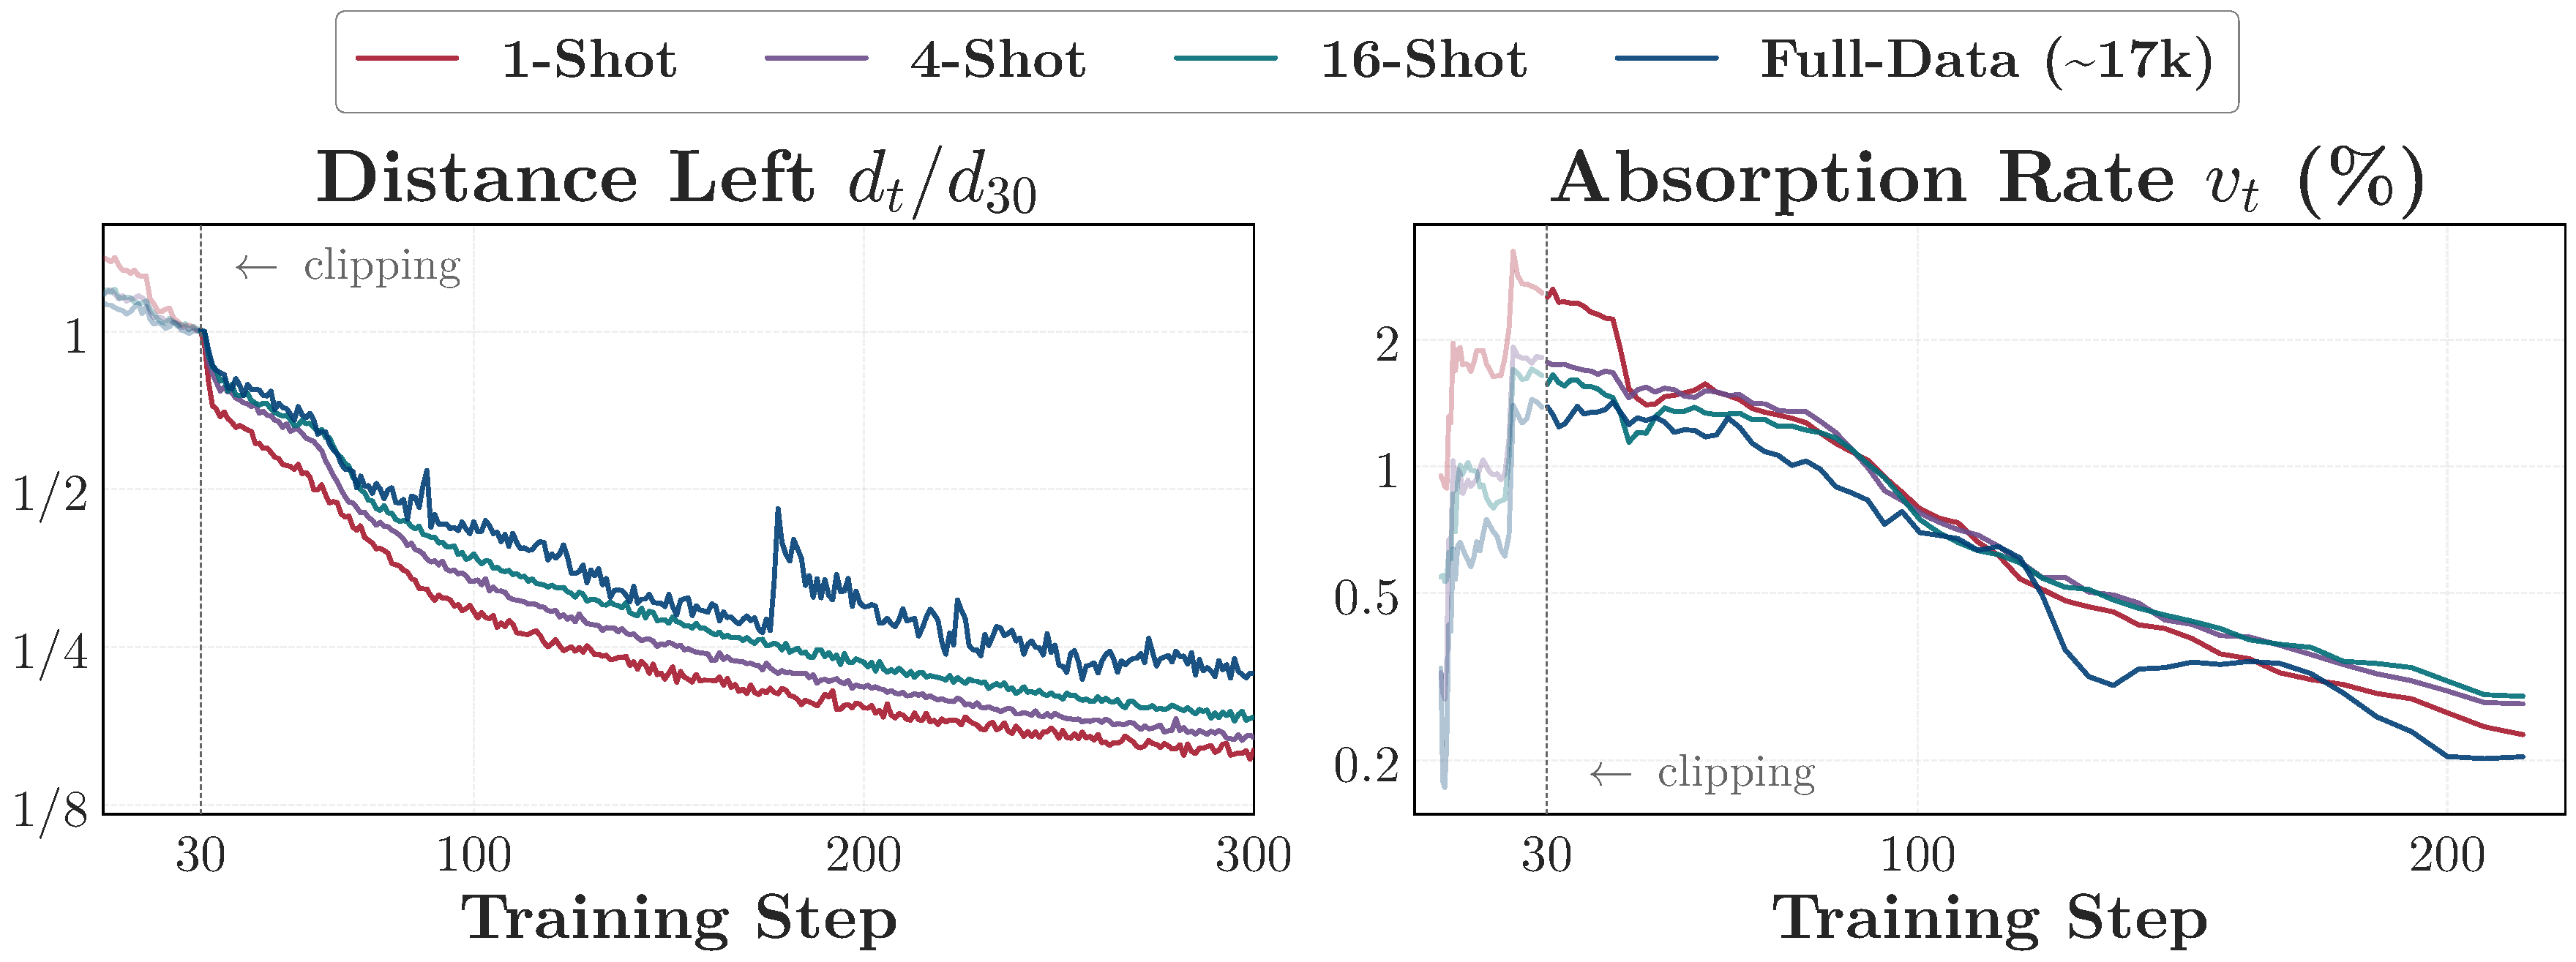
\includegraphics[width=0.75\linewidth]{figures/5_digestion_rate_v2.pdf}
    \caption{
    教师-学生对齐效果，针对在1、4、16及全部DAPO-Math-17k查询上训练的OPD。距离（左）和吸收率（右）均以对数刻度的纵轴相对于线性步长进行展示。
    }
    \label{fig:alignment-contraction}
\end{figure}

\paragraph{学生调整得越来越慢。}
距离在整个过程中持续下降，因此学生从未陷入停滞。减缓的是吸收速率，这在图~\ref{fig:alignment-contraction} 右侧面板中贯穿整个过程不断下降：在左侧的对数距离坐标轴上，恒定速率会呈现为一条直线，而所有四条曲线都变得更为平缓。因此每次更新所吸收的剩余量都比上次少，这就是为什么一次运行需要数百步而非数十步的原因。

\paragraph{吸收率在每个训练集大小下的下降方式大致相同。}
四次运行均以相同方式执行：每次在第 \(78\%\) 步到第 \(84\%\) 步之间，将第 \(30\) 步的距离减少 \(300\) 量，且四次运行在训练过程中均以相似的因子减慢（附录~\ref{app:alignment-dynamics} 提供了各次运行的具体数值以及这些读数所依据的约定）。因此，一次查询不会使对齐过程变慢或变快：速度是 OPD 的属性，而非训练集的属性。学习率仅影响所需步数的多少，而不影响距离下降的方式（附录~\ref{app:lr-sensitivity}）。

\subsection{固定状态下的消融分析}
\label{sec:fixed-states}
同策略训练会随着学生的变化不断产生新的状态，而对数百步的阅读表明，运行时间取决于这一状态供应的持续时间。将训练状态固定下来可以直接检验这一观点：如果一组固定的状态很快被耗尽，那么异策略运行就应该提前结束。

\paragraph{设置}
我们比较了两种仅在训练状态来源上不同的 one-shot 运行。始终同策略运行在每一步都从当前学生处获取新的轨迹。始终异策略运行则重复使用第~\ref{sec:state-diversity}~节中的 \(64\) 轨迹，这些轨迹仅从初始学生采样一次，用于每次更新，因此其训练状态保持固定，而学生则不断变化。

\paragraph{保持状态不变，运行时间仍然相同。}

\begin{figure}[t]
    \centering
    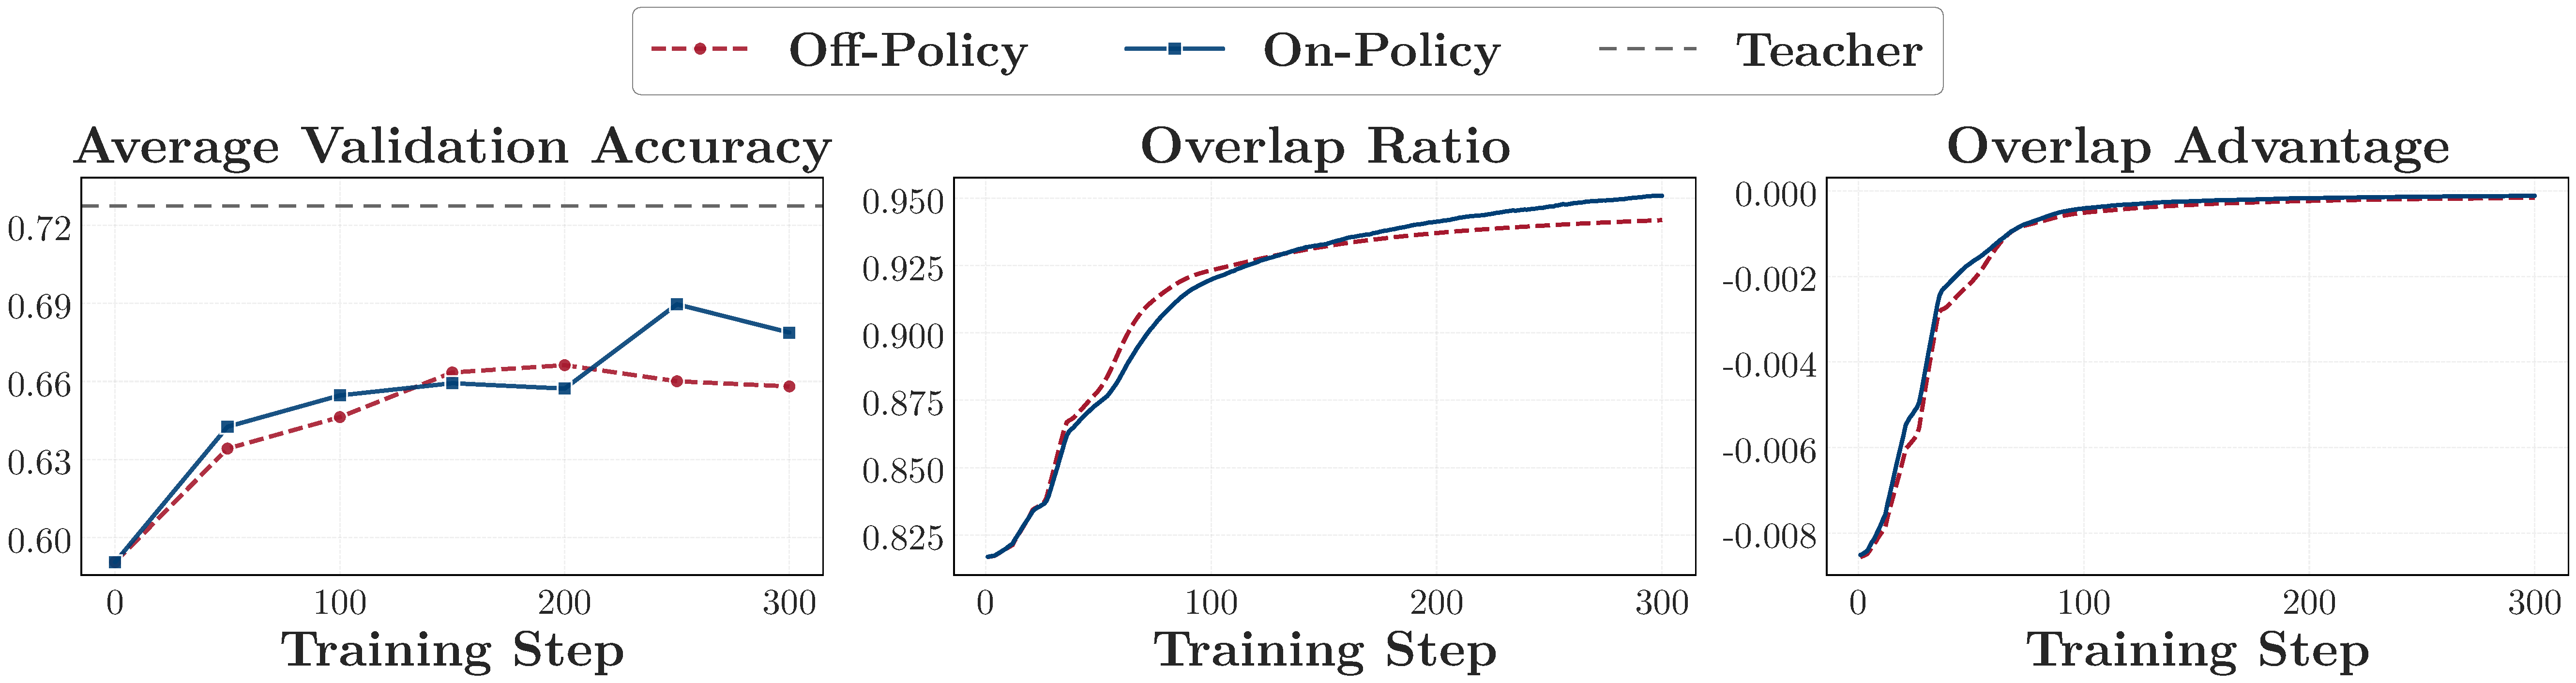
\includegraphics[width=\linewidth]{figures/5_online_offline.pdf}
    \caption{
    同策略和异策略 one-shot 运行的有效准确率和对齐度量。
    }
    \label{fig:online-offline}
\end{figure}
图~\ref{fig:online-offline} 显示，异策略运行的准确率在约 \(200\) 步内稳步提升，随后趋于停滞，因此其增益是在数百步内逐步累积的，而非仅在最初的几次更新中产生。对齐指标的变化同样缓慢：异策略运行的 top-\(16\) token 重叠率上升，且其重叠-token 优势趋近于零，均需经历数百步。因此，移除该状态供给并不会缩短运行长度。  
这表明，一组固定的状态本身已足以维持一次异策略动态（OPD）运行达数百步之久，故运行长度并非由新鲜状态持续到达的时间长短所决定。


\section{One-Shot 扩展至多教师 OPD}
\label{sec:mopd}

第~\ref{sec:state-diversity} 节表明，一个小型且语义多样的查询集可以在单一领域内达到全数据同策略蒸馏（OPD）的性能。现代后训练流水线通常使用\emph{多教师同策略蒸馏}（MOPD）~\citep{xiao2026mimo,xu2026deepseek}，其中学生模型在单次运行中对多个领域进行训练，每个查询被路由到其对应领域的教师模型。本节探讨的问题是：\textit{相同的查询多样性效果是否依然成立：对于每个领域，一个小型且多样化的查询集能否达到全数据MOPD的性能？}

\begin{tcolorbox}[takeawaysbox]
    每个领域内16个语义多样的查询就足以达到与全数据MOPD相当的性能，其平均验证准确率几乎与分离的全数据OPD相同。
\end{tcolorbox}

\begin{figure}[t]
    \centering
    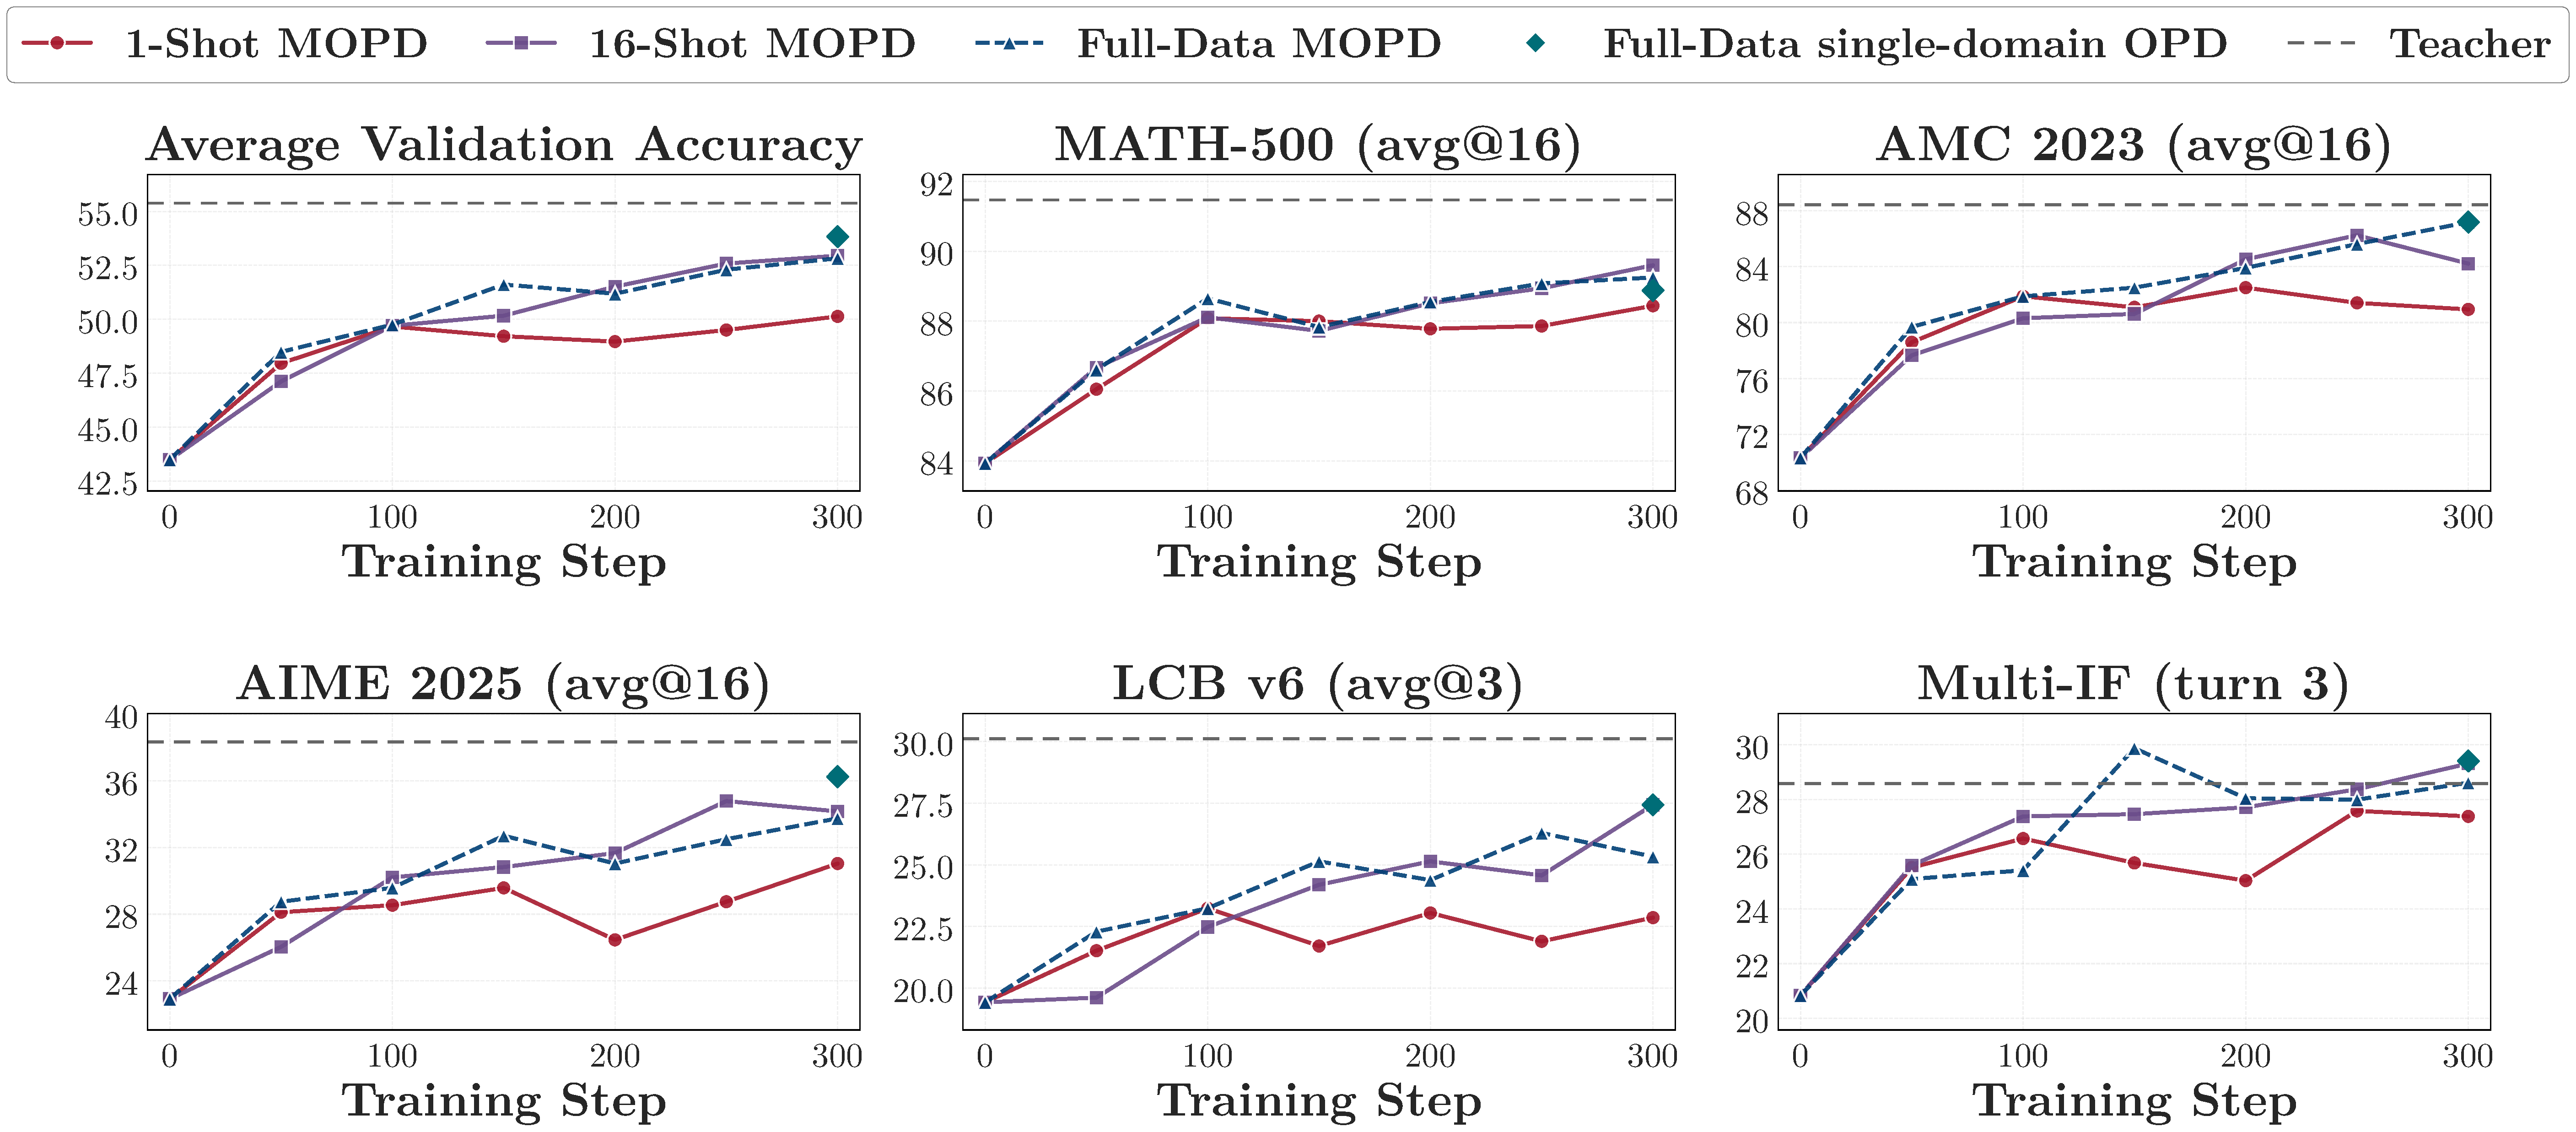
\includegraphics[width=\textwidth]{figures/6_mopd_curves.pdf}
    \caption{
    one-shot、16-shot 和全数据 MOPD 的验证准确率。
    }
    \label{fig:mopd}
\end{figure}

\paragraph{设置}
我们在数学推理、代码生成和指令遵循任务上，使用MOPD训练一个R1-Distill-1.5B学生模型。第\ref{sec:setup}节中的领域教师模型分别为：数学任务使用JustRL-1.5B，代码任务使用Nemotron-1.5B，指令遵循任务使用UltraData-IF-1.5B。我们排除了Agentic工具使用场景，因其采用了一个不同的学生模型Qwen-Coder-1.5B。这三种设置分别为one-shot、16-shot和全量数据MOPD。与第\ref{sec:state-diversity}节一致，16-shot设置从每个领域内分别拟合的16个BGE-M3~\citep{chen2024bge}语义簇中各选取一个代表性样本。所有设置均运行\(300\)步，所用超参数见表~\ref{tab:mopd-hyperparams}。

\paragraph{全数据MOPD与分离的全数据OPD相匹配。}
在步骤 \(300\) 时，全数据 MOPD 将平均验证准确率从 \(43.5\) 提升至 \(52.8\) ，恢复了教师-学生差距的 \(79\%\) 。三个对应的全数据 OPD 运行分别达到 \(53.8\) 。这一 \(1.0\) 点的差异表明，当三个领域在单次运行中同时训练时，MOPD 依然有效，并确立了全数据 MOPD 作为下文查询多样性比较的基准。

\paragraph{每个领域16个多样化查询即可匹配全数据MOPD。}
将每个领域的查询数量从1增加到16，使平均验证准确率在步骤\(300\)时从\(50.1\)提升至\(52.9\)。全数据MOPD达到\(52.8\)，因此16次查询MOPD恢复了全数据MOPD增益的\(101\%\)。该结果并非由单一领域驱动：分别计算，对应的比例分别为数学领域的\(93\%\)、代码生成领域的\(136\%\)以及指令遵循领域的\(109\%\)。由于16次查询和全数据MOPD使用相同的回滚和最优化预算，因此在此情景下，将每个领域的查询集扩展到超过16个多样化查询不会带来额外的平均增益。

这些结果共同支持了MOPD的状态空间解释：语义多样的查询可以在每个领域内引发互补状态，使得每个领域16个查询即可达到全数据MOPD的效果。




\section{讨论}
\label{sec:discussion}

上述机制将注意力从提示本身转移到提示所引发的推理状态区域。当学生的推演过程到达教师能够提供有效监督的区域时，输入才具有价值。陈述问题只是达到这些区域的一种方式。这一视角引出了两个更广泛的问题：输入本身需要包含多少任务内容？为什么相同的one-shot情景在OPD和RLVR下表现不同？我们通过分析内容稀疏和跨领域输入来探讨这些问题，随后与one-shot RLVR进行受控对比。

\subsection{输入作为状态生成器}
\label{sec:template}

状态生成器视角认为，如果输入仍能引发教师可监督的轨迹，则任务内容可能是不必要的。我们通过一个以 \texttt{<think>} 结尾的空用户回合、相同模板搭配简单领域系统提示，以及来自 WildChat~\citep{zhao2024wildchat} 的通用领域查询（图~\ref{fig:template-examples}）来验证这一预测。WildChat 数据集包含 \(192{,}824\) 个主要为英文的通用对话、创意写作、角色扮演和改写类查询。保守性启发式仅将 \(0.17\%\)  标记为与数学相关，\(2.63\%\)  标记为与代码相关。

\begin{figure}[t]
\centering
\begin{minipage}[t]{0.485\textwidth}
\begin{tplbox}{(a) Base template}
\begin{tplinput}
\ttfamily\scriptsize\raggedright \tplctrl{<|begin\_of\_sentence|>}\tplrole{<|用户|>}\tplthink{思考}\tplesc{\textbackslash n}
\end{tplinput}
\end{tplbox}
\end{minipage}\hfill
\begin{minipage}[t]{0.485\textwidth}
\begin{tplbox}{(b) System template --- Code}
\begin{tplinput}
\ttfamily\scriptsize\raggedright \tplctrl{<|begin\_of\_sentence|>}解决编程竞赛问题。从标准输入读取，向标准输出写入。\tplrole{<|User|>}\tplthink{<|think|>}\tplesc{\textbackslash n}
\end{tplinput}
\end{tplbox}
\end{minipage}
\\[4pt]
\caption{用于OPD训练输入的两个内容稀疏模板。}
\label{fig:template-examples}
\end{figure}

\begin{figure}[t]
\centering
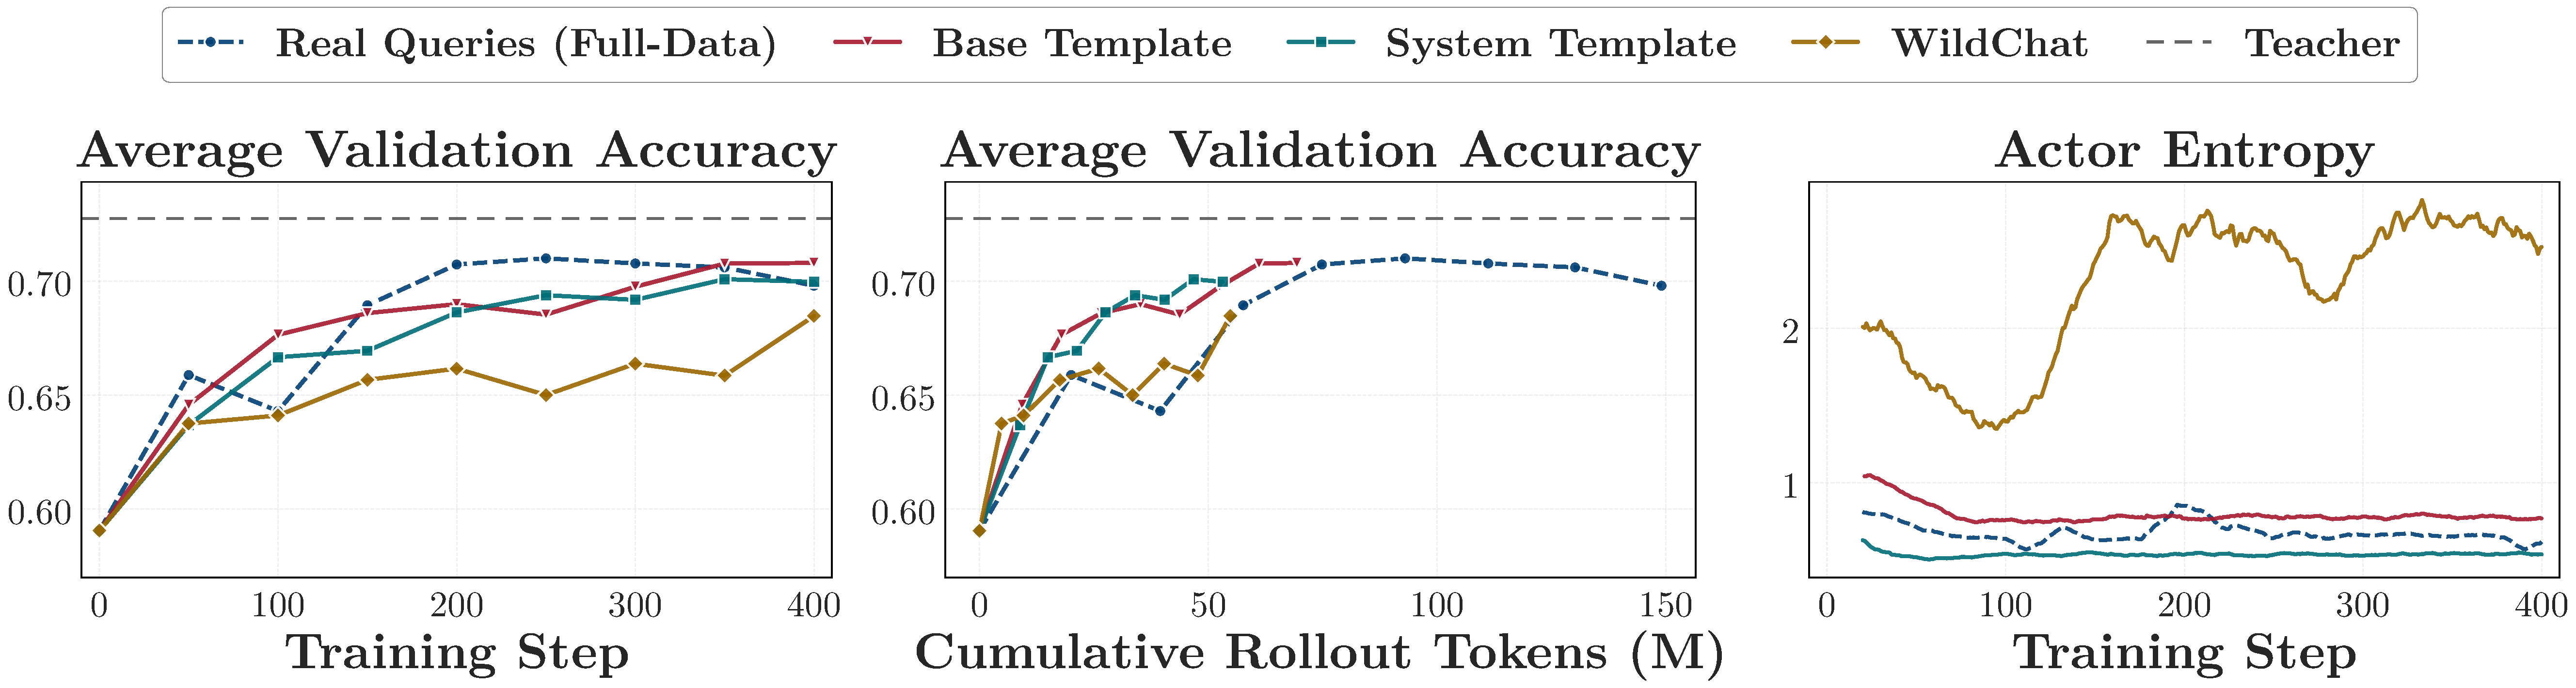
\includegraphics[width=\textwidth]{figures/7_template_wildchat.pdf}
\caption{
在真实训练集、内容较少的模板或通用领域WildChat查询上训练的数学OPD的有效准确率和演员熵。
}
\label{fig:template-wildchat}
\end{figure}

\paragraph{内容稀疏且跨领域的输入仍能引发有用的状态。}
所有三个条件均追踪真实查询基准（real-query baseline），使三个基准的平均值从 \(59.1\) 提升至 \(69.8\)，且三者均在 rollout token 总量的三分之一到二分之一处即达到该水平（图~\ref{fig:template-wildchat}）。代码生成任务亦呈现相同趋势（附录~\ref{app:template-code}）。  
然而，该要求并非空洞：一种能立即闭合该块的支架（scaffold），即 \texttt{<think>\\n}\allowbreak\texttt{</think>\\n}，会坍缩为简短的元层级回复，而此类回复无法用于训练。  
这些结果并不意味着任务内容通常可有可无；相反，它们表明内容并非 OPD 中有用信号的唯一来源。输入本身亦充当状态生成器，即使内容稀疏或来自非目标领域（off-domain）的输入，有时亦可引导学生进入支持有效教师监督（teacher supervision）的状态。在本实验中，显式领域内容（explicit domain content）的改变仅使最终性能波动约一个百分点。这为理解 OPD 的数据效率提供了互补视角：数据质量不仅取决于所收集问题本身，还取决于这些问题所诱导出的状态区域（state regions），以及在这些区域内可获得的教师目标（teacher targets）。

\subsection{与one-shot RLVR的关系}
\label{sec:opd-vs-rlvr}

one-shot OPD 与 one-shot RLVR~\citep{wang2025oneshot} 具有相同的表面现象：单次查询即可支持在 OPD 中经过数百次更新的持续改进，以及在 RLVR 中经过上千次更新的持续改进。其学习来源不同：OPD 在每个访问的状态下接收教师目标，而 RLVR 则为每条轨迹接收可验证的结果。我们通过相同的中等复杂度查询来比较二者，以隔离这一差异（图~\ref{fig:opd-vs-rlvr}）。

\begin{figure}[t]
\centering
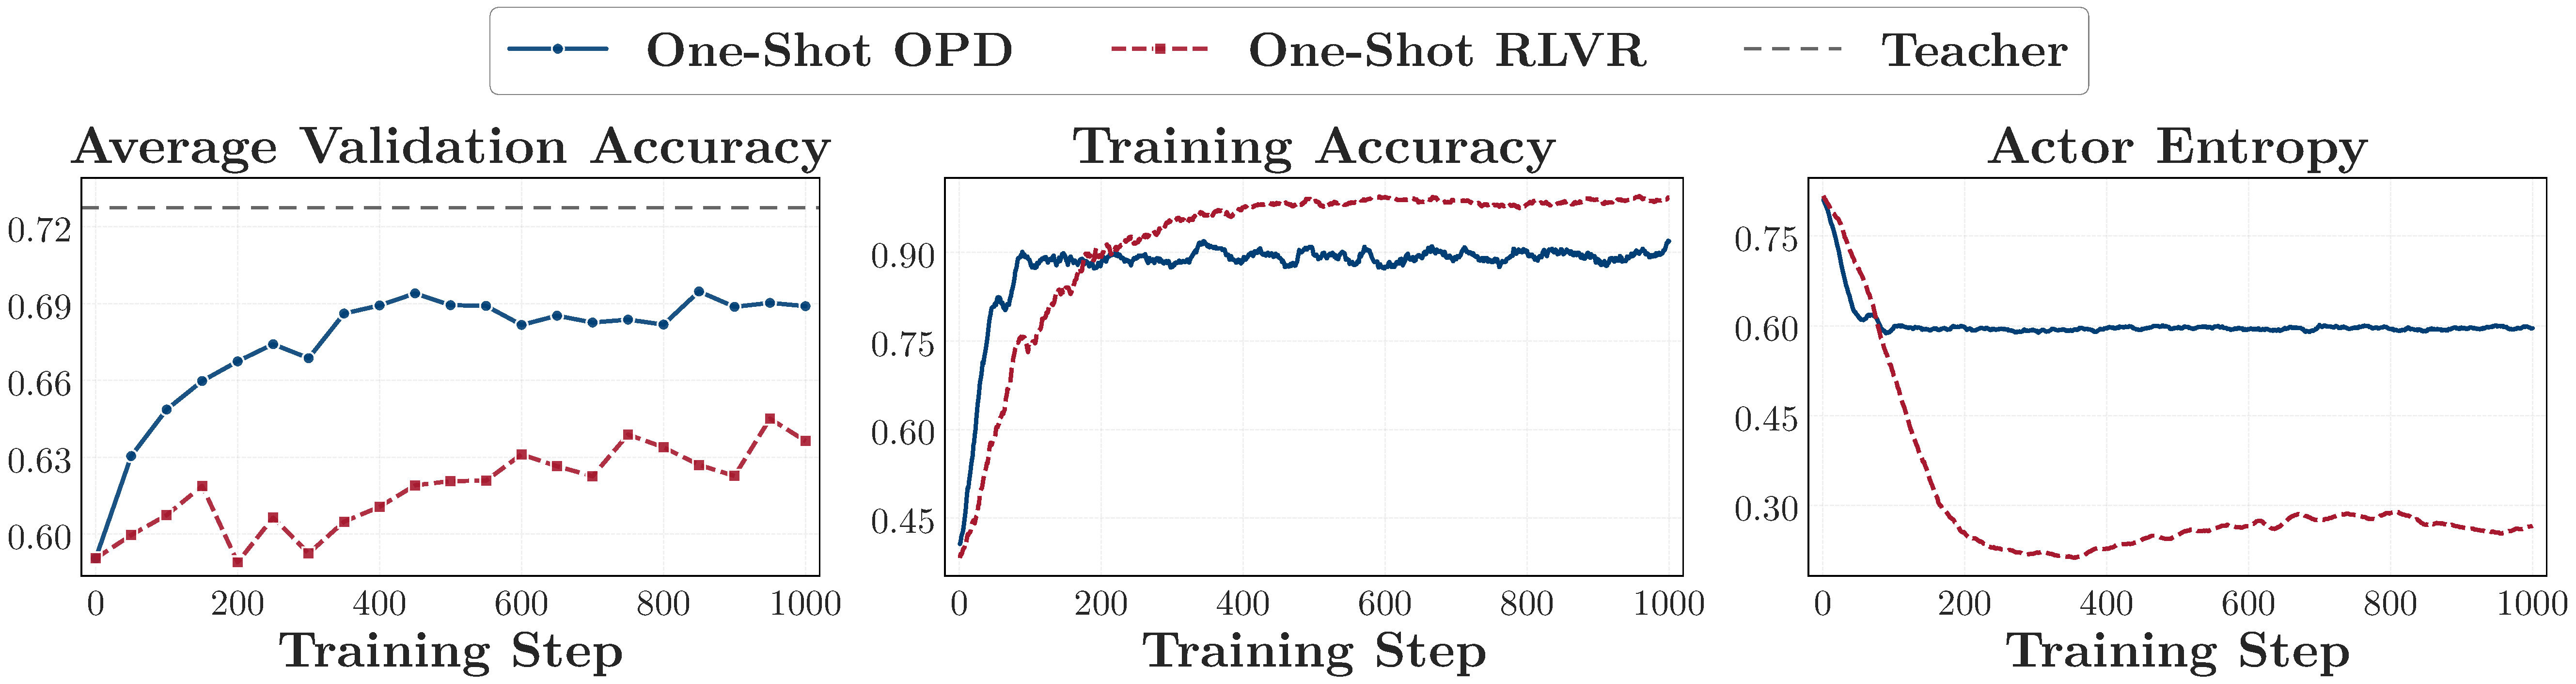
\includegraphics[width=\textwidth]{figures/7_opd_vs_rlvr.pdf}
\caption{
有效准确率和训练动态在相同查询下的 one-shot OPD 与 one-shot RLVR。两者每步均处理批量 \(64\)  查询。RLVR 每个查询抽取 \(8\)  轮次，并根据 GRPO 下的结果对每轮进行评分。OPD 抽取 \(1\)  并对每个采样 token 与教师进行对比评分。训练准确率是解决训练查询的轮次所占比例。
}
\label{fig:opd-vs-rlvr}
\end{figure}

\paragraph{有用的输入因目标而异。}
RLVR 从轨迹结果中进行更新。因此，其训练输入必须定义一个任务，使得采样的结果可以被验证。这些结果还必须具备足够的变化性，以产生有用的优势。而 OPD 则从每个访问状态下的教师-学生差距中进行更新。只要某个提示导致轨迹暴露出此类差距，它就能接收到有用的信号。因此，OPD 输入的价值并不直接依赖于可验证性或难度。我们的结果进一步表明，即使在我们研究的情景中，较弱的领域对齐也能发挥作用。诱导状态区域的覆盖仍然重要（第~\ref{sec:data} 节），但获得这种覆盖所需的限制远低于获得具有可验证结果的任务。

\paragraph{OPD 从同一查询中提取了更多信号。}
两个算法在每一步都从训练查询中获取新的轨迹。在 \(1000\) 步内，OPD 缩小了与教师模型之间差距的 \(72\%\)。其验证准确率的提升是 RLVR 的两倍以上。当两种方法按轨迹 token 数量而非训练步数进行匹配时，这一优势依然存在（图~\ref{fig:opd-vs-rlvr}）。

随着模型学会解决训练查询，RLVR 信号会逐渐减弱。其组别很快变得几乎一致，这使得在 GRPO 下无法获得优势。OPD 不依赖于轨迹结果的变化。即使在查询被解决后，它仍能从局部的教师-学生差距中继续学习，尽管这些差距逐渐缩小。因此，one-shot RLVR 的局限性在于其查询所能提供的结果变化；而 one-shot OPD 的局限性则在于其吸收稠密教师监督的速度，如第~\ref{sec:data} 和~\ref{sec:algorithm} 节所示。此外，两种目标也意味着不同的上限：RLVR 不受教师分布的限制，而 OPD 则被训练以匹配某一特定分布。


\section{相关工作}
\label{sec:related}

\paragraph{同策略蒸馏}
同策略蒸馏（OPD）在教师监督下使用自身的轨迹训练学生模型~\citep{song2026survey}。MiniLLM~\citep{gu2024minillm} 通过策略梯度在反向 KL 下优化了这一过程，而 GKD~\citep{agarwal2024policy} 将其泛化至散度以及同策略与异策略混合情形。\citet{yang2026learning} 将 OPD 视为稠密 KL 约束的强化学习，其中每个 token 的对数比率充当隐式奖励。如今，OPD 出现在前沿的后训练架构中~\citep{yang2025qwen3,zeng2026glm,xiao2026mimo,xu2026deepseek,blakeman2026nemotron}，其中若干采用我们在第~\ref{sec:mopd} 节研究的多教师形式，将每个查询路由至领域专家。越来越多的研究从算法层面解释了为何 OPD 有效：一条主线研究其目标与更新几何结构：稠密的 per-token 目标取代了结果奖励强化学习中的单个序列级标量，这在参数空间中引导一个早期锁定、低秩的更新子空间~\citep{cai2026learning,shen2026geometry}，且可重述为 token 级策略梯度~\citep{ko2026scaling}，从而与将 SFT 的稠密更新与 RL 的局部子网络分离的分析相连接~\citep{mukherjee2026reinforcement,zhu2025path}。另一条主线则探讨 OPD 成功或失败的条件：教师与学生间共享的思维模式，以及教师过强的局限性~\citep{li2026rethinking}，哪些 token 实际上可被学习~\citep{armandpour2026unmasking,wang2026not}，以及具有简单修复方案的反复失败模式~\citep{zhu2026many,fu2026revisiting}。这些解释均以训练集为给定前提。我们则提出：OPD 需要多少训练输入？并发现关键约束并非数据量，而是学生吸收信息的速率。

\paragraph{数据高效的推理后训练。}
一条并行的研究探讨了少量数据如何激发强大的推理能力。在稀疏结果-奖励强化学习情景下，\citet{wang2025oneshot} 表明单个示例能够使模型持续优化超过一千步，我们将其适配到 OPD 的稠密信号设置中。LIMR~\citep{limr} 通过评估每个示例的学习影响进行排序，将 RLVR 训练集剪枝数倍。在监督微调下，LIMA~\citep{zhou2023lima}、LIMO~\citep{ye2025limo} 和 s1~\citep{muennighoff2025s1} 仅需约千个精心筛选的示例，即可获得具有竞争力的对齐或推理能力。在 OPD 中，对推理前缀调度监督可使训练成本降低数倍~\citep{zhang2026fast}。更广泛的后训练工作则通过影响度或质量来选择高价值子集~\citep{xia2024less,chen2024alpagasus,he2025right,he2025air}。这些工作与我们的数据效率主题一致，但其监督仍依赖于精心筛选的问题，在强化学习情况下以稀疏结果标量形式提供，或在 SFT 情况下以参考解形式提供。而 OPD 则在每个访问的前缀处提供稠密的 per-token 目标，并在学生从未解决过的查询上依然有效（第~\ref{sec:one-shot} 节），即使在错误的滚动路径上，教师信号仍保持信息丰富~\citep{armandpour2026unmasking}，因此限制因素从是否存在有用信号这一在稀疏奖励下的固有难题，转变为同策略学生吸收已充足信号的速度（第~\ref{sec:mech-dynamics} 节）。

\paragraph{合成的无监督后训练数据。}
越来越多的研究工作减少了后训练对人工编写、精心筛选数据的依赖。其中一个方向是对输入进行合成：Self-Instruct~\citep{wang2023self} 和 Evol-Instruct~\citep{xu2024wizardlm} 从语言模型中引导生成指令，而 Magpie~\citep{xu2025magpie} 仅凭一个聊天模板前缀即可激发完整的“指令—响应”对。第二个方向则在强化学习（RL）~\citep{he2026far} 中去除真实标签，以模型置信度或熵~\citep{zhao2026learning,agarwal2026unreasonable} 等自生成信号、多条 rollout 中的多数一致结果~\citep{zuo2026ttrl}，或从未标记语料库~\citep{dong2025reinforcement} 中提取的奖励，替代可验证的奖励。第三个方向则彻底摒弃外部任务，让模型自行提出任务~\citep{zhao2026absolute,zweiger2026self}。这些研究路径分别放松了对奖励或查询来源的监督要求。我们的模板驱动及 WildChat-OPD 实验结果（第~\ref{sec:template} 节）进一步推动了查询侧的解耦：由于教师模型在每个访问到的前缀处均提供稠密监督，查询的作用仅在于将学生模型置于一种有益的推理状态，因此一个跨领域聊天日志，甚至一个无内容的模板，均可近乎同样有效地驱动 OPD。
\section{结论、局限性与未来工作}
\label{sec:conclusion}
\label{sec:limitations}

\paragraph{结论。} 
受 one-shot RLVR~\citep{wang2025oneshot} 的启发，我们提出了一个问题：单次查询是否也足以实现 OPD？答案是肯定的：one-shot OPD 能使学生在数百步内持续提升，并恢复绝大部分全数据 OPD 所带来的收益，跨越不同模型家族和任务领域。数据与算法两个层面给出了统一的答案：OPD 存在数据过载但算法匮乏的问题。一次查询通过其轨迹所到达的状态作用于学生，而单次查询已覆盖全数据 OPD 所访问的大部分状态空间；16 个语义多样化的查询在单领域 OPD 和 MOPD 中均能实现与全数据训练相当的效果。限制运行时长的因素是吸收率：每次更新所吸收的剩余教师-学生差距比例持续下降，无论是一次查询还是全部 17k 次查询，其下降速度一致，因此决定运行时长的是优化器而非训练集。输入只需启动学生的推理过程，这使得数据设计从收集问题转变为选择教师。

\paragraph{局限性。}
状态覆盖是基于全数据回放构建的参考空间进行语义层面的代理度量，它报告的是查询集达到该空间的程度，而非其自身所覆盖的内容，且对每个簇赋予相等权重，无论该簇被访问的频率如何，或仍携带多少教师信号。吸收率的决定因素尚不明确。我们的MOPD运行使用了三个领域，每个领域对应一个教师，因此随着教师数量的增加，多样性结果能扩展到何种程度仍不清楚。

\paragraph{未来工作。}
三个方向依次如下。
\begin{itemize}[topsep=2pt, partopsep=0pt, leftmargin=12pt, itemsep=2pt]
    \item 按状态覆盖选择数据：问题不再是如何收集查询数量，而是这些查询引发哪些状态，因此一旦能够从查询本身估算出状态覆盖，而无需通过完整数据运行来测量，状态覆盖便成为一种选择准则。
    \item 通过在每个token的差距信任区域下，重复使用批量数据进行多轮训练，或根据token所携带的教师信号量对其进行加权，从而提高训练的步骤效率。
    \item 扩展情景，涵盖更多教师和领域，以及更大规模的学生、Agentic 工具使用和长上下文，这些场景下训练数据的收集成本最高。
\end{itemize}

\bibliography{main}

\newpage
\clearpage
\appendix
\section{第~\ref{sec:one-shot}~节的详细信息}

\subsection{实验设置与训练查询}
\label{app:model-data}

\paragraph{遵循指令的设置。}
\label{app:IF-setup}
与其他主领域教师不同，指令遵循教师模型是专门为我们的实验训练的。我们从 DeepSeek-R1-Distill-Qwen-1.5B 出发，在具有可编程验证约束的合成指令遵循任务上对该模型进行后训练。我们采用 GRPO 方法，并使用基于规则的结果奖励，以指示响应是否满足目标轮次约束。训练时每个提示生成四个补全，温度设为 \(0.9\)；最大提示长度为 \(4{,}096\) 个 token，最大响应长度为 \(16{,}384\) 个 token；优化器采用 AdamW，学习率为 \(1\times10^{-6}\)，训练批量大小为 \(16\)，裁剪比为 \(0.2\)。第 600 步的检查点被用作指令遵循教师模型，使 IFBench \citep{pyatkin2026generalizing} 从 \(14.33\) 提升至 \(20.65\)，Multi-IF 最终轮次准确率从 \(20.84\) 提升至 \(28.58\)。

对于该领域，“full-data”表示从 UltraData-SFT-2605 \citep{ultradata-sft-2605} 中采样的子集，而非完整数据集，且 one-shot 查询随机从中选取。


\paragraph{针对 one-shot OPD 的数学查询（表~\ref{tab:one-shot-queries}，图~\ref{fig:probe_prompt_training_acc}）。}
\label{app:training-accuracy}
我们从未经训练的学生模型中为 DAPO-Math-17K 的前 64 个查询中的每一个采样 8 次轨迹，并根据最终通过率分配难度，从而选定 \texttt{t59} (\(8/8\) )、\texttt{t22} (\(4/8\) ) 和 \texttt{t56} (\(0/8\) ) 分别作为简单、中等和困难的查询。在训练过程中，每个查询被解决的频率符合这一分配：简单查询始终维持在 \(1.0\) 左右，中等查询从 \(0.36\) 上升至约 \(0.89\) ，而困难查询在 \(300\) 步内从未被解决，然而如图~\ref{fig:probe_prompt} 所示，这三个查询均带来了相近的基准提升。

\begin{table}[t]
    \centering
    \small
    \setlength{\tabcolsep}{4pt}
    \begin{tabular}{p{0.10\textwidth}p{0.08\textwidth}p{0.74\textwidth}}
    \toprule
    Difficulty & ID & Query \\
    \midrule
    Easy & \texttt{t59} &
    In triangle \(ABC\), let \(D\) be the foot of the altitude from \(A\). Suppose that \(AD=4\), \(BD=3\), \(CD=2\), and \(AB\) is extended past \(B\) to a point \(E\) such that \(BE=5\). Determine the value of \(CE^2\). \\
    \midrule
    Medium & \texttt{t22} &
    Let \(S\) be the set of triples \((a,b,c)\) of non-negative integers such that \(a+b+c\) is even. Determine the value of
    \(\sum_{(a,b,c)\in S} \frac{1}{2^a3^b5^c}\).
    This sum can be expressed as \(\frac{m}{n}\), where \(m\) and \(n\) are relatively prime positive integers. Compute \(m+n\). \\
    \midrule
    Hard & \texttt{t56} &
    Byan is playing a game called ``raven, raven, falcon'' with his three friends. His friends sit in a circle, and Byan walks clockwise around them, tapping each friend he passes on the head and saying either ``raven'' or ``falcon,'' each with probability \(\frac{1}{2}\). The game ends when Byan has said ``falcon'' twice. The probability that one of his friends will be called a ``falcon'' twice can be expressed as \(\frac{m}{n}\), where \(m\) and \(n\) are relatively prime positive integers. Find \(100m+n\). \\
    \bottomrule
    \end{tabular}
    \caption{在查询难度实验中使用的数学查询，按学生在OPD训练前的通过率进行标签标注。}
    \label{tab:one-shot-queries}
\end{table}

\begin{figure}[t]
    \centering
    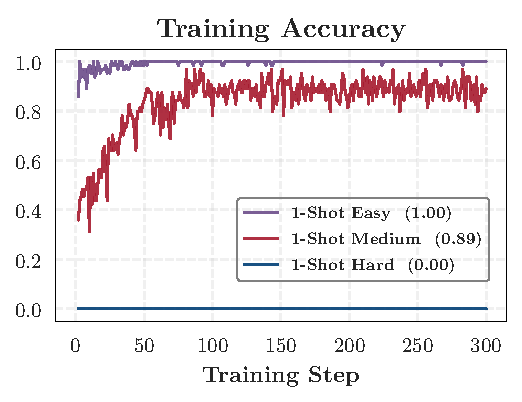
\includegraphics[width=0.45\linewidth]{figures/3A_ablations_training_acc.pdf}
    \caption{每个步骤中，64次滚动采样中有多少比例能够解决训练查询本身，针对表~\ref{tab:one-shot-queries}中的三个查询。}
    \label{fig:probe_prompt_training_acc}
\end{figure}

\paragraph{OPD 的默认超参数（表~\ref{tab:opd-hyperparams}）。}
除非另有说明，所有实验均使用以下默认设置。top-\(K\) 行涵盖了两个目标：第~\ref{sec:finding-recovery}~节中的数学 one-shot 运行使用 \(K=16\) ，而所有其他实验均使用采样 token 目标。

\begin{table}[t]
\centering
\caption{OPD的默认超参数。}
\label{tab:opd-hyperparams}
\small
\begin{tabular}{ll}
\toprule
\textbf{Item} & \textbf{Value} \\
\midrule
Rollout batch size      & 64 \\
Mini batch size         & 64 \\
Responses per prompt    & 1 \\
KL coefficient          & 0.0 \\
LogProb top-$K$         & 0(default) / 16 \\
Top-$K$ strategy        & Student Top-$K$ \\
Loss aggregation        & token-mean \\
Training temperature    & 1.0 \\
Top-$p$                 & 1.0 \\
Optimizer               & AdamW ($\beta_1{=}0.9$, $\beta_2{=}0.999$, wd $=0.01$) \\
Learning rate           & 1e-6 \\
Gradient clip norm      & 1.0 \\
Max prompt length       & 1024 (math); 4096 (code, IF, agentic) \\
Max response length     & 7168 (math, code, IF); 2048 (agentic) \\
\bottomrule
\end{tabular}
\end{table}


\section{第~\ref{sec:data}~节的详细信息}

\subsection{训练状态覆盖}
\label{app:state-coverage}
\label{app:state-coverage-robustness}

\paragraph{建设。}
每个优化步骤收集轨迹而非随机收集，以确保训练的每个阶段都得到同等表示，且各情景下的预算具有可比性，这些情景均运行相同步数：在完整数据运行的从 \(1\) 到 \(500\) 每一步中，我们获取 \(5\) 条轨迹，其中三条用于构建簇，两条构成完整数据（保留）部分，共 \(12{,}000\) 条参考状态和 \(8{,}000\) 条保留状态。通过PAC将这些轨迹降维至 \(50\) 维，保留 \(71.9\%\) 的方差，再进行 \(K\) -均值聚类。随后，对每个评估情景均按相同调度进行测量，在每一步抽取 \(2\) 条来自 \(5\) 条轨迹的样本，并在整个训练过程中累积，使得第 \(300\) 步的预算 \(600\) 条轨迹与保留分割相匹配。该抽样过程重复 \(30\) 次；带状区域和误差条表示这些重复结果的标准差，反映了轨迹下采样带来的差异，而非不同训练模型之间的变化。

\paragraph{该排序在 \(K\) 、参考构建以及状态位置上均保持稳定（表~\ref{tab:coverage-k} 和~\ref{tab:coverage-reference}，图~\ref{fig:state-position-sensitivity}）。}
覆盖度取决于参考状态的聚类精细程度以及定义簇的状态，因此我们同时改变这两个因素。第一张表重复了分析，\(K\in\{50,100,200,500\}\) 时更细的簇导致绝对覆盖度降低，但覆盖度仍从1-shot到4-shot再到16-shot逐步提升，16-shot接近全数据情况。第二张表则基于每个情景下\(2{,}000\) 次滚动结果的并集重建簇，而非仅基于全数据状态，其排序依然成立；由于来自所有情景的状态共同定义了这些合并簇，合并覆盖度并非恢复度量，其各行仅应相互比较。图中改变了从每次滚动读取的位置，将最终非填充token与固定绝对位置\(2{,}000\) 和\(4{,}000\) 与主分析中的8个相对位置进行对比。四种情况均保持了相同排序。固定位置变体的结果接近主构造，而最终token在查询较少时给出显著更低的覆盖度，这正是由响应长度和终止决定位置所预期的结果；因此我们采用8个相对位置，可对任意长度的响应进行全程采样。

\begin{table}[t]
    \centering
    \small
    \caption{全数据锚定训练状态覆盖，步骤 \(300\)  下不同簇数量 \(K\)  时。}
    \label{tab:coverage-k}
    \begin{tabular}{lcccc}
        \toprule
        \(K\)
        & 1-shot
        & 4-shot
        & 16-shot
        & Full data (held-out) \\
        \midrule
        50  & 0.755 & 0.829 & 1.000 & 1.000 \\
        100 & 0.727 & 0.803 & 1.000 & 1.000 \\
        200 & 0.715 & 0.798 & 0.989 & 1.000 \\
        500 & 0.564 & 0.695 & 0.904 & 0.956 \\
        \bottomrule
    \end{tabular}
\end{table}

\begin{table}[t]
    \centering
    \small
    \caption{在不同簇构造下的训练状态覆盖，当 \(K=200\) 时。}
    \label{tab:coverage-reference}
    \begin{tabular}{lcccc}
        \toprule
        Reference construction
        & 1-shot
        & 4-shot
        & 16-shot
        & Full data (held-out) \\
        \midrule
        Full-data anchored
        & 0.663 & 0.773 & 0.953 & 0.998 \\
        Equal-size pooled
        & 0.750 & 0.845 & 0.958 & 0.966 \\
        \bottomrule
    \end{tabular}
\end{table}

\begin{figure}[t]
    \centering
    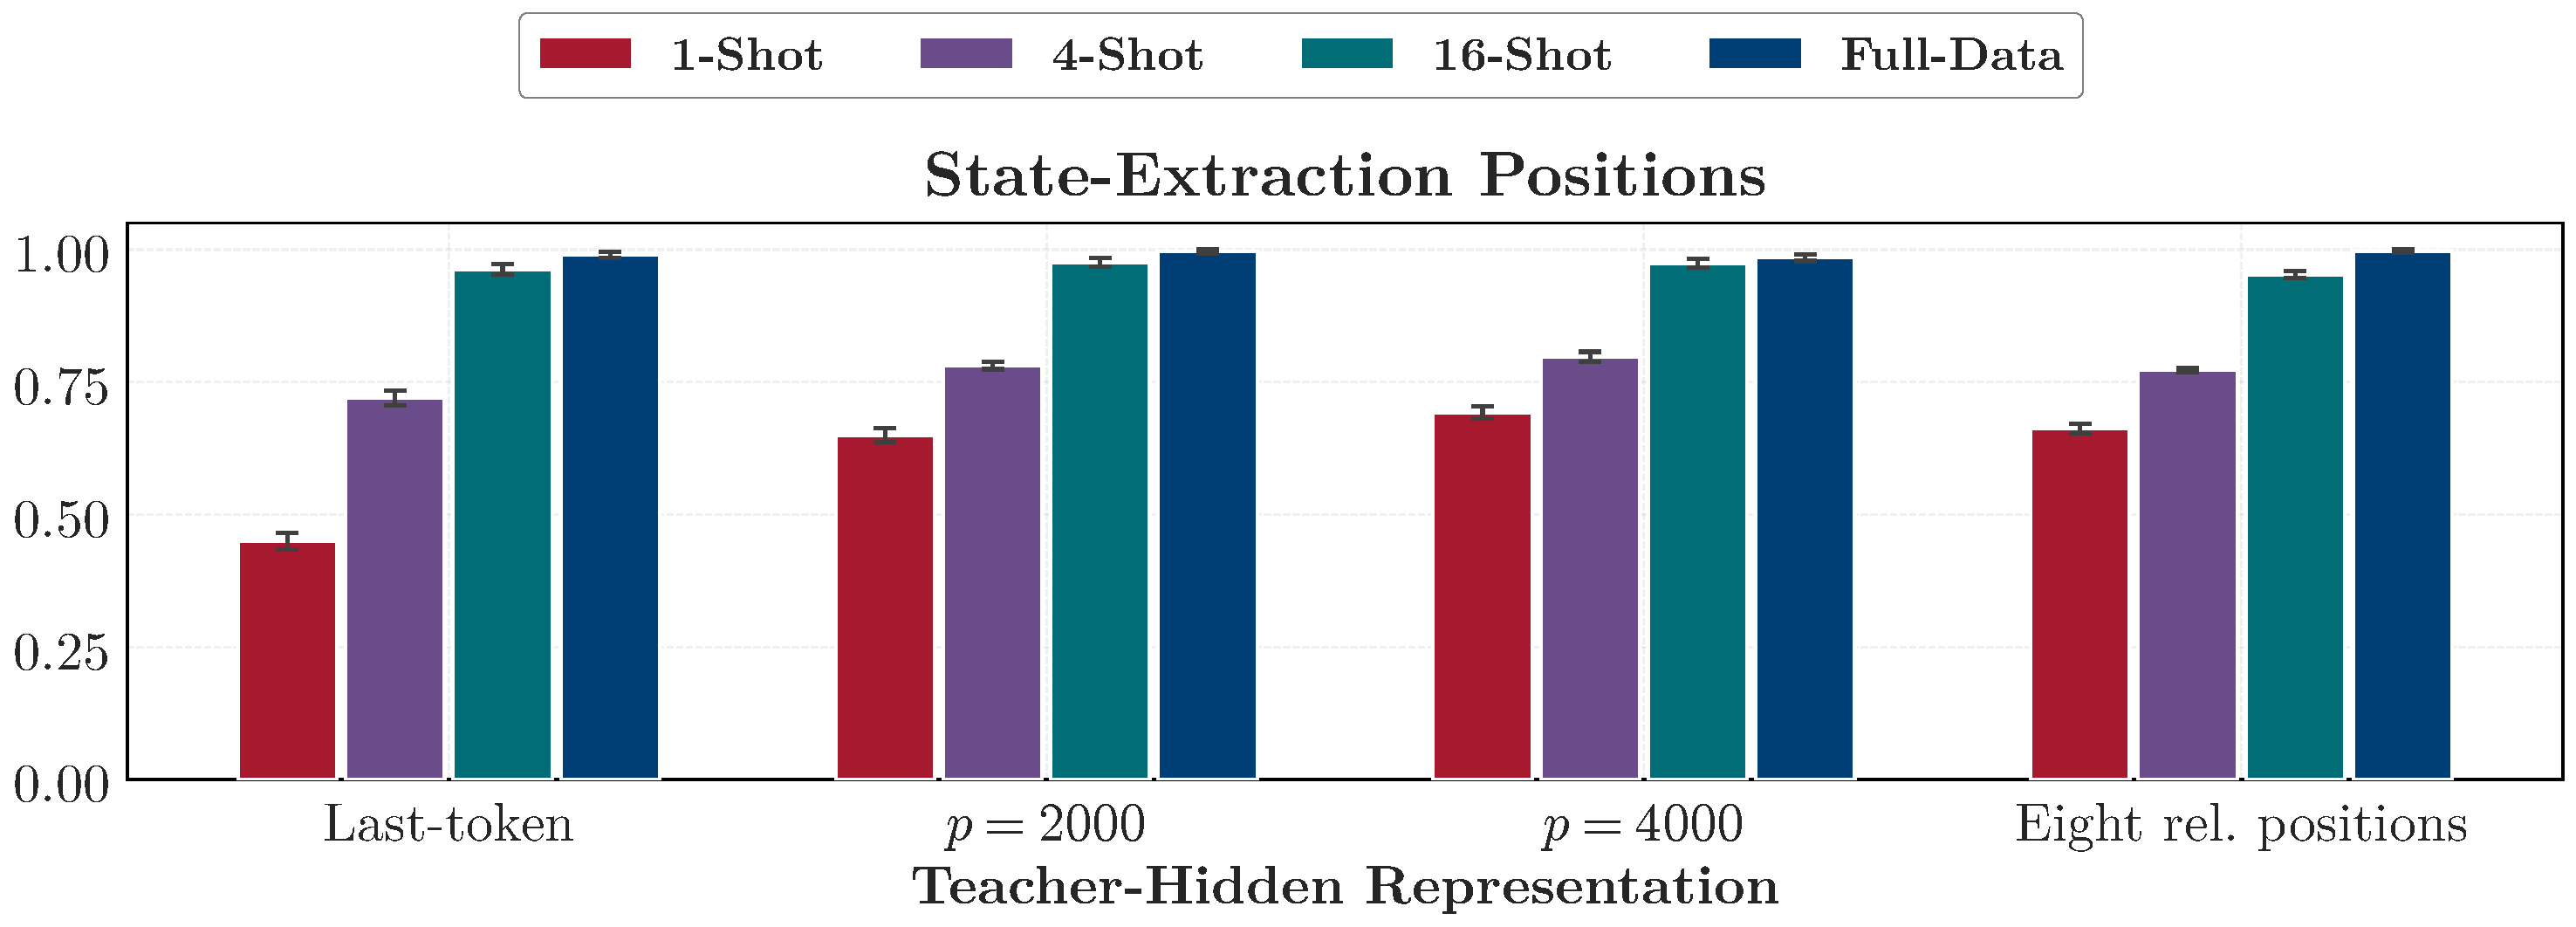
\includegraphics[width=0.85\linewidth]{figures/4A_state_extraction_positions.pdf}
    \caption{在不同状态提取位置下的训练状态覆盖，对应 \(K=200\)。误差条表示滚动子采样的一标准差。}
    \label{fig:state-position-sensitivity}
\end{figure}

\paragraph{one-shot 具有更重的远距离状态尾部，但与完整数据不可分离（表~\ref{tab:reference-diagnostics}）。}
最近质心分配将一个状态分配到某个簇中，即使它与所有全数据状态的距离都很远，因此仅靠覆盖无法区分参考空间填充稀疏的情景与填充较密的情景。因此，我们还测量每个状态在未缩减的 \(1536\) 维空间中与其十个最近参考状态的平均余弦距离，并在该距离超过保留样本中全数据状态的 \(95\) 百分位数时，将该状态标记为非参考状态。one-shot OPD 超过阈值的频率高于其他情景，因此其距离分布的上尾更重。然而，与保留的全数据状态相比，其 AUROC 为 \(0.552\)，接近随机水平，说明 one-shot 状态整体上不可分离于全数据状态。

\begin{table}[t]
    \centering
    \small
    \caption{不同查询集大小下的参考距离诊断。AUROC 将每个情景与保留的完整数据状态进行比较。最后一行是包含构建簇所用回放数据的完整数据池，因此其超过率无需等于 \(5\%\)  所设定的阈值。}
    \label{tab:reference-diagnostics}
    \begin{tabular}{lccc}
        \toprule
        Setting
        & Exceedance (\%)
        & Mean distance
        & AUROC \\
        \midrule
        1-shot   & 17.2 & 0.283 & 0.552 \\
        4-shot   & 4.4  & 0.218 & 0.477 \\
        16-shot  & 3.8  & 0.231 & 0.512 \\
        Full data (all)  & 4.0  & 0.215 & 0.476 \\
        \bottomrule
    \end{tabular}
\end{table}

\subsection{训练数据的控制}
\label{app:fixed-count-diversity}
\label{app:schedule}

\paragraph{16-shot OPD 中的多样性（图~\ref{fig:fixed-count-diversity}）。}
阶梯中第~\ref{sec:state-diversity}~节的每个查询代表一个不同的语义簇，因此同时提升了多样性和数量。保持数量为16，并从单一簇中抽取第二组数据进行分离：这16个簇代表在步骤~\(300\)~处达到~\(70.9\)~的有效准确率，而单一簇组仅为~\(69.9\)~，这大约相当于4次采样OPD使用四分之一查询量所达到的水平，其状态覆盖也以相同方式分离，并且更早实现，~\(98.9\%\)~，而单一簇组在~\(76.8\%\)~附近趋于平坦，仅在~\(100\)~步内完成。来自单一簇的查询会不断将学生带回其已访问过的状态空间部分。

\begin{figure}[t]
  \centering
  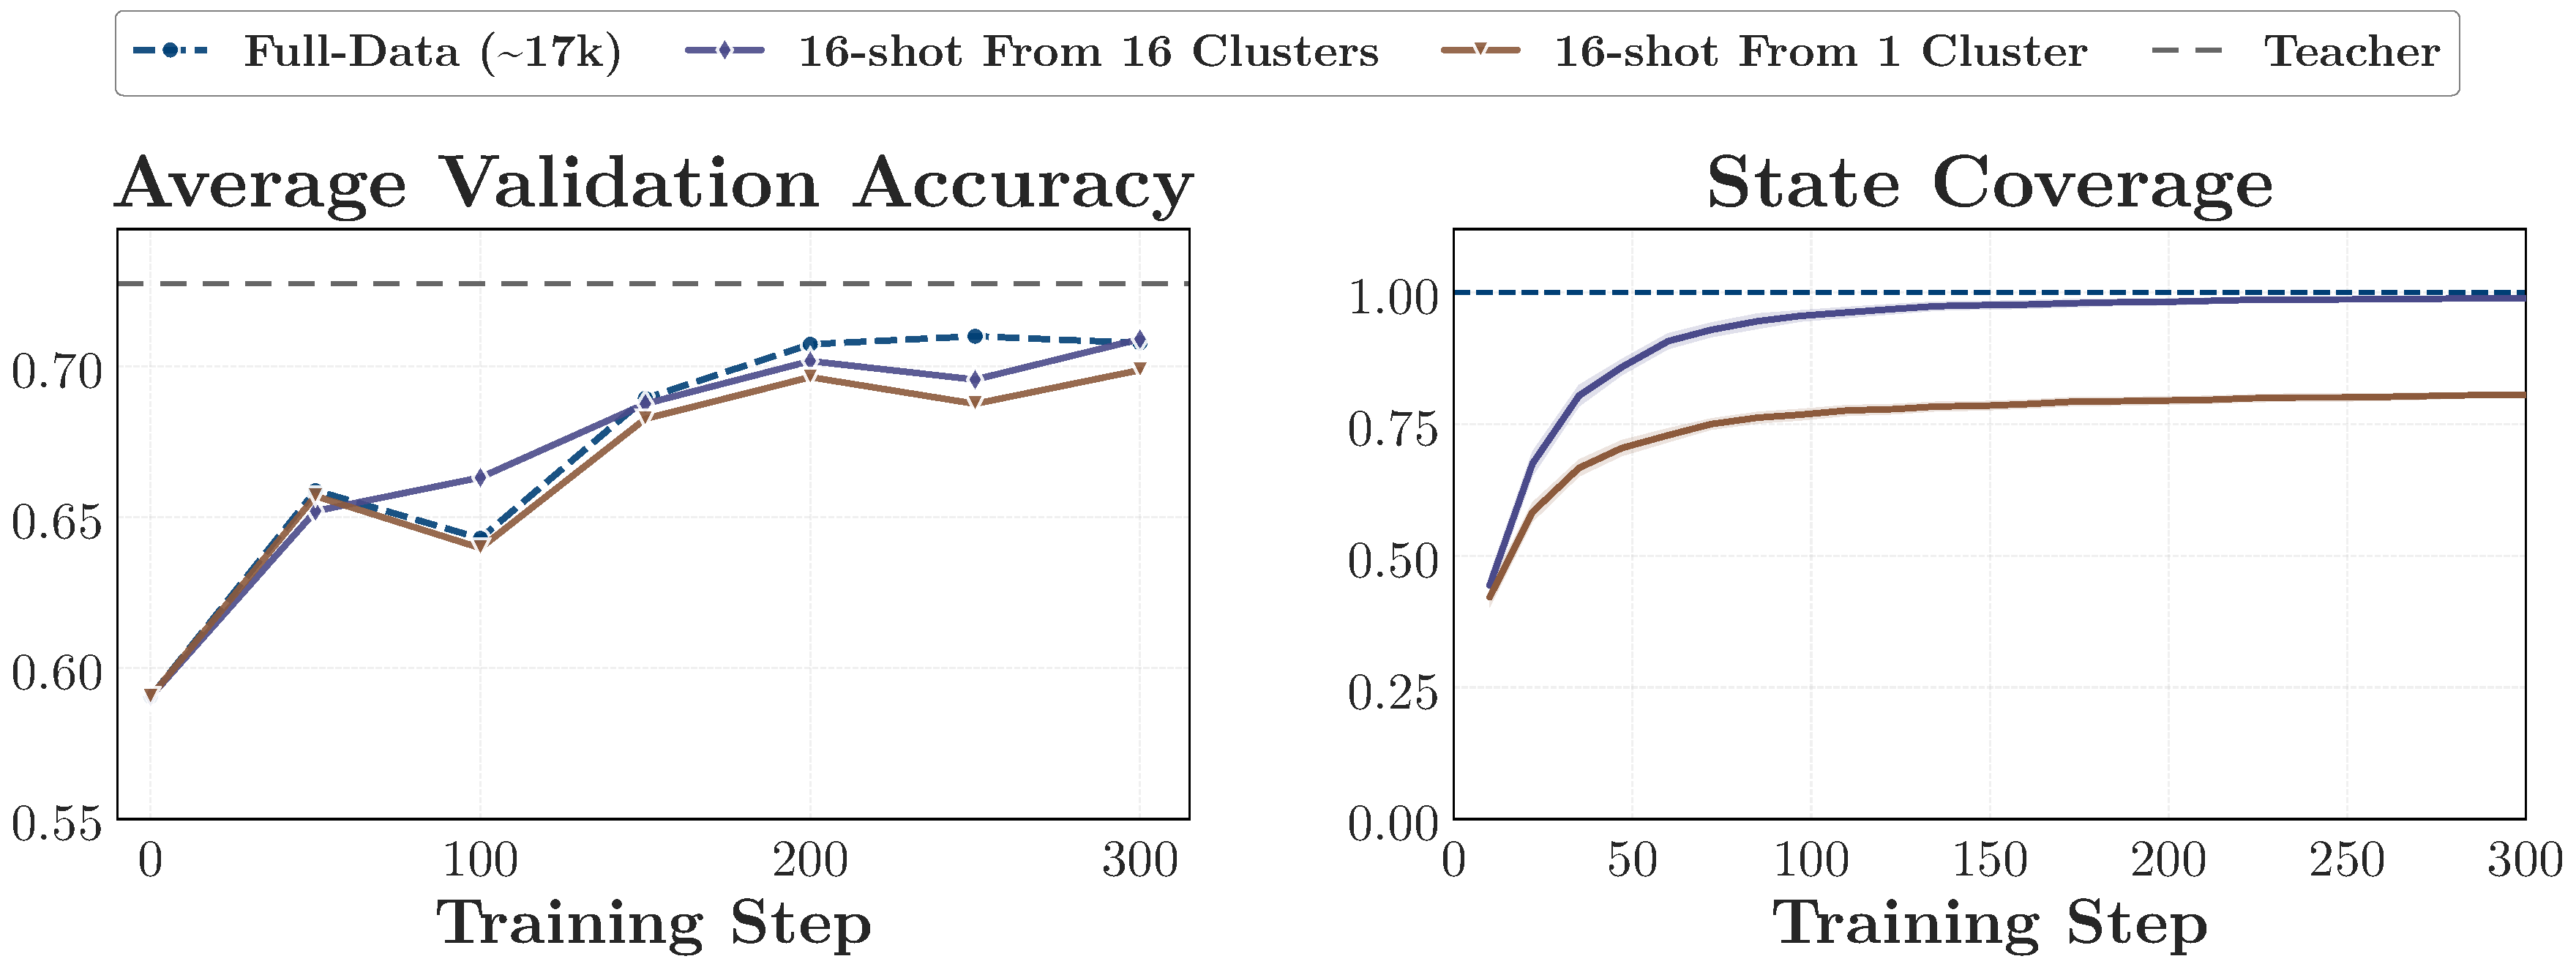
\includegraphics[width=0.75\linewidth]{figures/4A_nshot_diversity.pdf}
  \caption{两个仅在多样性上不同的16次查询集，与全数据OPD进行对比。}
  \label{fig:fixed-count-diversity}
\end{figure}

\paragraph{在 2 次查询 OPD（图~\ref{fig:nshot_schedule}）中的查询调度。}
固定一个双查询集，仅改变每个查询的呈现时机：顺序调度在 \(600\) 步预算的前 \(300\) 步上训练困难查询，剩余步数则训练中等难度查询；而混合调度则在每个批量中各放入 \(32\) 份困难查询和中等难度查询。在第 \(600\) 步时，二者分别达到 \(68.8\) 和 \(69.1\) ，均高于它们共享的 one-shot 基准的 \(67.4\) ，因此，在第二个查询本身所带来的收益面前，对固定查询集进行排序几乎无关紧要。这些实验的训练时长远超第~\ref{sec:state-diversity} 节中的实验，并以困难查询作为其基准，故其时间范围（horizon）与基准均不可与图~\ref{fig:state-diversity} 中的结果互换。

\begin{figure}[t]
  \centering
  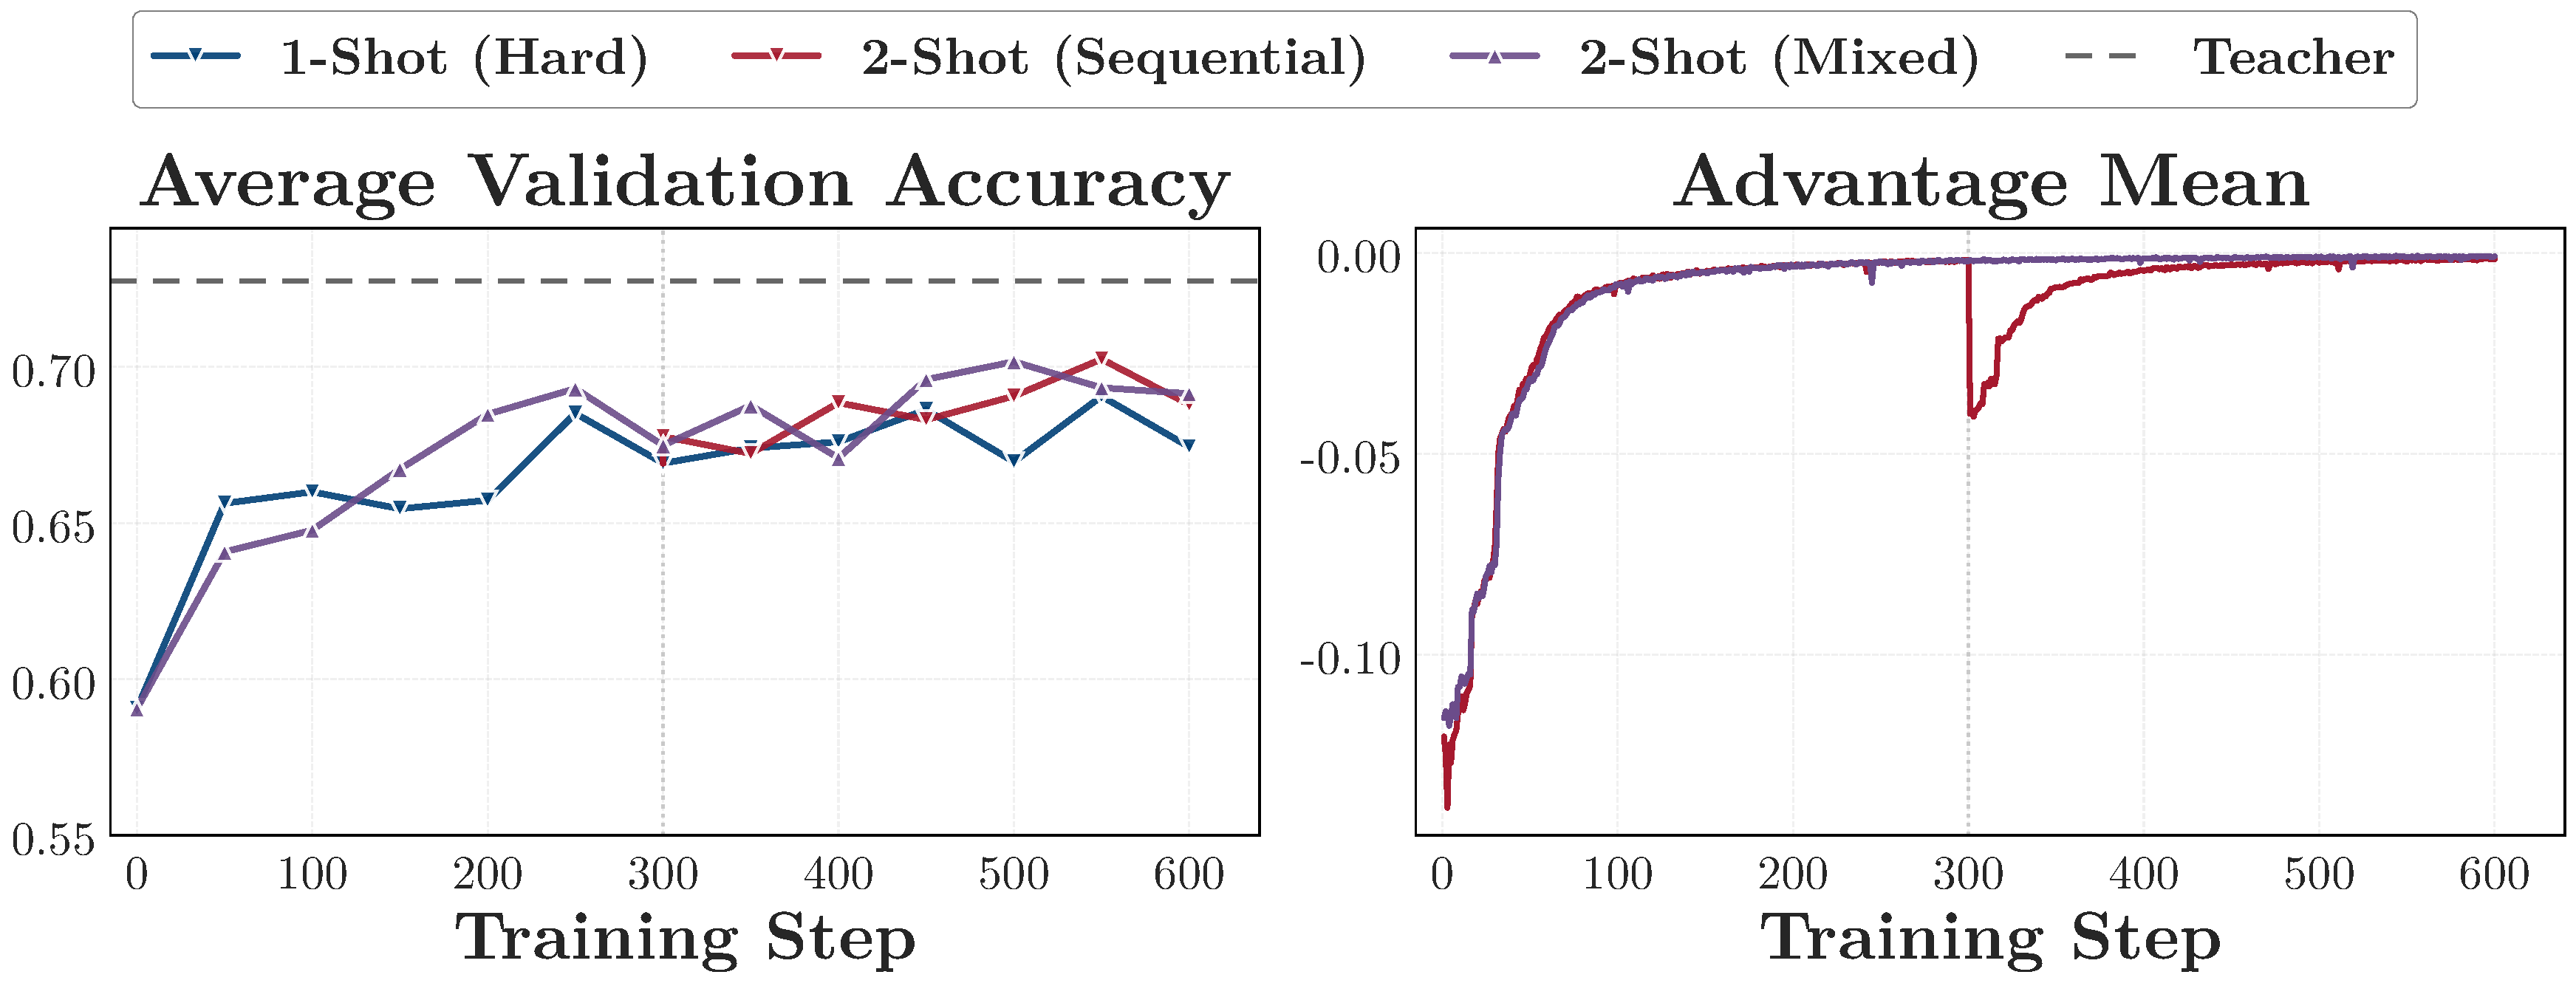
\includegraphics[width=0.75\linewidth]{figures/4A_2shot_schedule.pdf}
  \caption{2-shot OPD中查询调度的影响。垂直虚线标记了顺序调度中的查询切换点。}
  \label{fig:nshot_schedule}
\end{figure}

\section{第~\ref{sec:algorithm}~节的详细信息}

\subsection{估算吸收率和测量窗口}
\label{app:alignment-dynamics}

第~\ref{sec:mech-dynamics} 节在三种不同约定下进行测量。为何每一种：
\begin{itemize}[topsep=2pt, partopsep=0pt, leftmargin=13pt, itemsep=2pt, parsep=0pt]
    \item  \(\boldsymbol{[t/1.4,\,1.4t]}\) . 当 \(d\)  缓慢移动时，相邻步长之间的差异主要为噪声，因此 \(v_t\)  被视为该窗口两端点间 \(\log d\)  的斜率，使用每个端点附近的中位数 \(d\)  进行计算。仅当窗口完全位于测量值域内的中心点才会被绘制，这也是主文中读取步骤 \(50\)  和 \(200\)  的速率，而非步骤 \(300\)  的原因。
    \item  \(\boldsymbol{d_t/d_{30}}\)。每次运行测量其访问状态的距离，四个在每一步上处于不同层级 \(30\)，因此将其各自值绘制在对应位置，可使曲线通过形状而非层级进行比较。
    \item  \textbf{从步骤 \(30\) 开始。} 梯度裁剪在此前一直有效，而裁剪后的更新并非目标所要求的更新：\(v_t\) 在该窗口内衡量的是一个\emph{固定大小}步长所带来的收益，而非一个步长所带来的收益，这就是为什么在该处测量到的速率上升而非下降的原因。
\end{itemize}

表~\ref{tab:gap-reduction} 汇总了第~\ref{sec:mech-dynamics} 节引用的该值域中的数据：在步骤 \(300\) 时，步长-\(30\) 距离剩余的比例，以及步骤 \(50\) 与 \(200\) 之间吸收率下降的因子。

\begin{table}[t]
    \centering
    \small
    \caption{同策略 OPD 在默认学习率下的步数对齐动态 \(30\) --\(300\)。}
    \label{tab:gap-reduction}
    \begin{tabular}{lcccc}
        \toprule
        Setting (queries) & 1 & 4 & 16 & Full data \\
        \midrule
        \(d_{300}/d_{30}\) & 0.16 & 0.17 & 0.18 & 0.22 \\
        \(v_{50}/v_{200}\) & 5.6 & 5.2 & 4.2 & 6.4 \\
        \bottomrule
    \end{tabular}
\end{table}

\subsection{学习率重新缩放了步长轴}
\label{app:lr-sensitivity}

我们重复同策略 one-shot OPD，分别在半倍、默认以及两倍于默认学习率的情景下进行，保持其他所有设置不变，并在同一 \(300\) 步数范围内读取全部三种情况的结果，如第~\ref{sec:mech-dynamics} 节所述。

\begin{figure}[t]
    \centering
    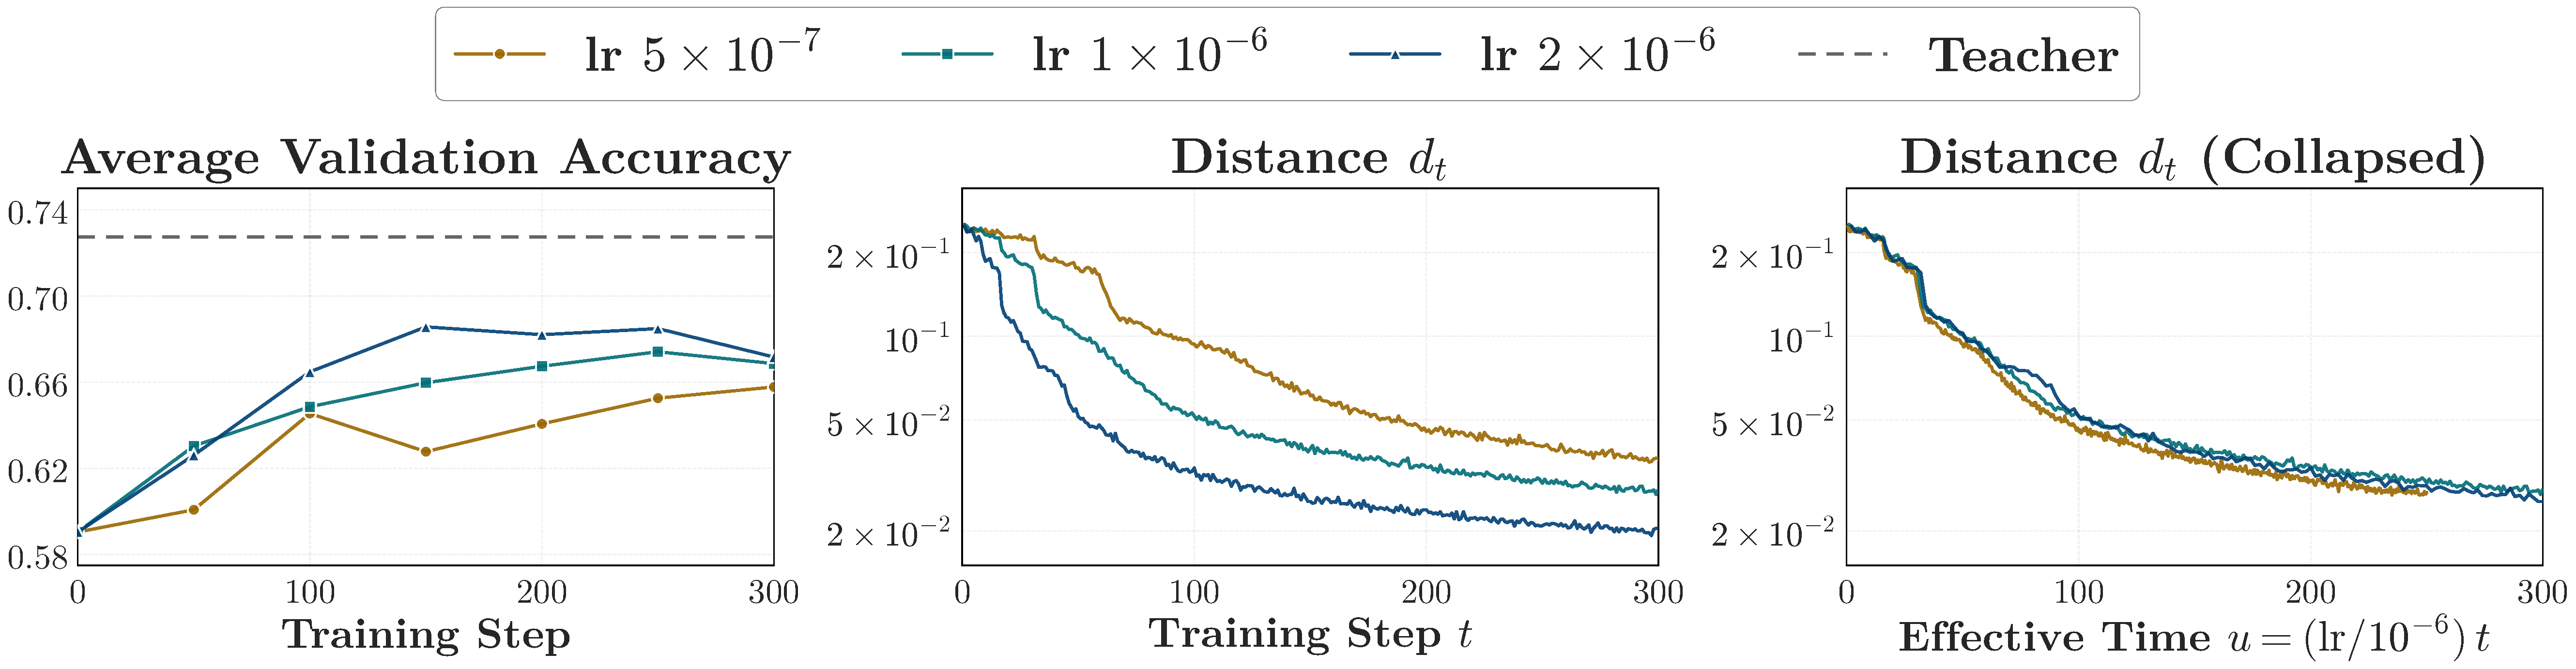
\includegraphics[width=\linewidth]{figures/5A_lr_collapse_v2.pdf}
    \caption{one-shot OPD 在一半、正常和两倍默认学习率下的验证准确率与教师-学生距离。距离以对数刻度的纵轴表示，时间以线性刻度表示。}
    \label{fig:lr-sensitivity}
\end{figure}

\paragraph{学习率会缩放步长轴，而保持减速部分不变。}
较大的学习率会更早达到任意给定的距离，三条曲线之间的分离程度大致与学习率的比值成比例（图~\ref{fig:lr-sensitivity}）。将横轴从步数 \(t\) 改为 \(u=(\mathrm{lr}/10^{-6})\,t\) 后，它们便重合为一条曲线：三次运行之间的差距从约 \(2.2\times\) 缩小到约 \(1.1\times\)。因此，学习率仅决定了运行沿该曲线移动的速度，而不会改变曲线本身的形状。随着距离增加，曲线变得越来越平坦，正如第~\ref{sec:mech-dynamics} 节中四种查询情景相对于步数的表现一样。因此，在我们测试的四倍范围中，成比例更大的学习率会成比例地缩短运行时间，而不会触及导致对齐变慢的初始原因。


\section{第~\ref{sec:mopd}~节的详细信息}
表~\ref{tab:mopd-hyperparams} 显示了MOPD的默认超参数。

\begin{table}[!ht]
\centering
\caption{MOPD（多教师同策略蒸馏）的默认超参数。}
\label{tab:mopd-hyperparams}
\small
\begin{tabular}{ll}
\toprule
\textbf{Item} & \textbf{Value} \\
\midrule
Number of teachers      & 3 (math / code / IF) \\
LogProb top-$k$         & 0  \\
KL coefficient          & 0.0 \\
Loss aggregation        & seq-mean-token-mean \\
\midrule
Rollout batch size      & 64 \\
Mini batch size         & 64 \\
Responses per prompt    & 1 \\
Training temperature    & 1.0 \\
Top-$p$                 & 1.0 \\
\midrule
Optimizer               & AdamW ($\beta_1{=}0.9$, $\beta_2{=}0.999$, wd $=0.01$) \\
Learning rate           & 1e-6 \\
Gradient clipping       & 1.0 \\
\midrule
Max prompt length       & 4096 \\
Max response length     & 7680 \\
\bottomrule
\end{tabular}
\end{table}


\section{第~\ref{sec:discussion}~节的详细信息}

\subsection{代码生成中的模板与WildChat OPD}
\label{app:template-code}

第~\ref{sec:template} 节报告了数学中的四种输入条件。此处我们报告代码生成中的相同四种条件。

\paragraph{设置}
该学生模型为 R1-Distill-1.5B，教师模型为 DeepCoder-1.5B-Preview~\citep{deepcoder2025}，基准模型为 TACO~\citep{li2023taco} 上的全数据 OPD。基础模板、系统模板和 WildChat 查询与第~\ref{sec:template} 节中的完全一致；系统模板中的一行指令为图~\ref{fig:template-examples}b 中的竞赛编程指令。我们在 LiveCodeBench v6 上以 avg@3 为评估指标进行评测。

\begin{figure}[!htb]
  \centering
  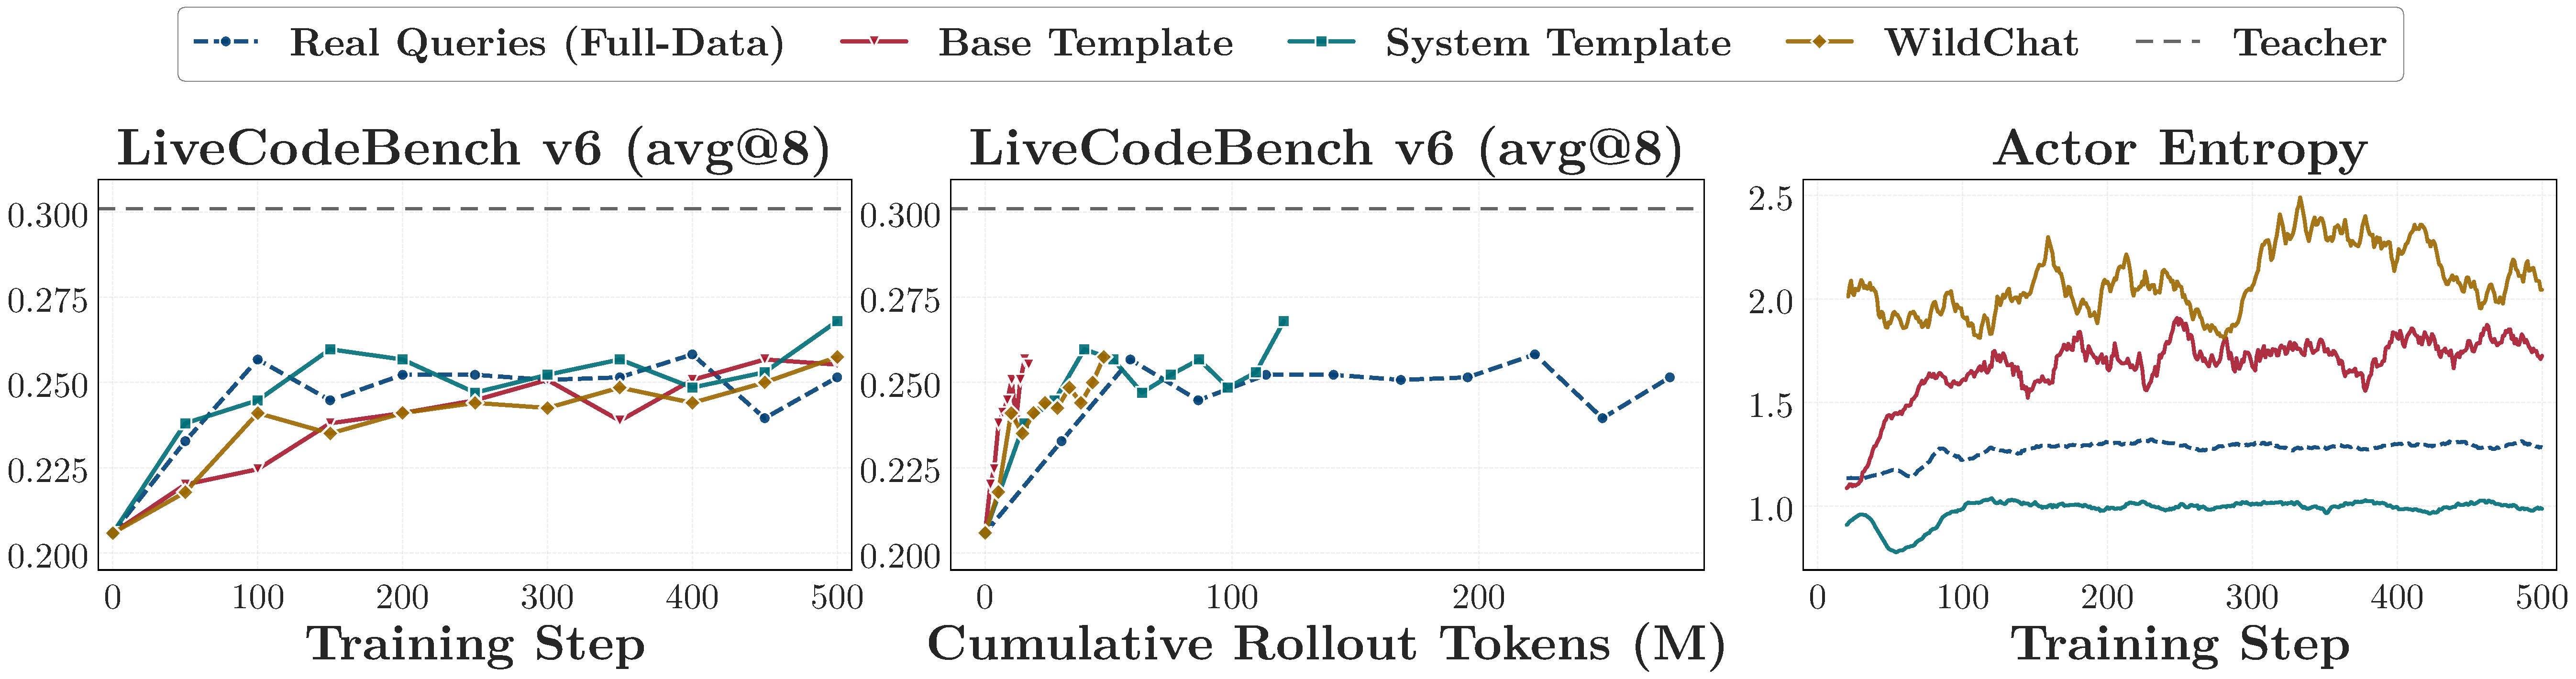
\includegraphics[width=\textwidth]{figures/7A_template_wildchat_code.pdf}
  \caption{代码生成OPD的验证准确率和演员熵。
  }
  \label{fig:template-wildchat-code}
\end{figure}

\paragraph{结果。}
图~\ref{fig:template-wildchat-code} 显示了四种情况结束时彼此之间的差距在 \(1.7\) 以内，而 token 计算方式将它们分隔得比步数计算方式远得多：在相同的 \(500\) 步内，基准方案消耗了 \(277\) M 的回放 token，而基础模板为 \(18\) M，其余两种情况介于两者之间。演员熵的排序与数学中的顺序完全一致，其中 WildChat 最高，系统模板最低。唯一的不同是此处没有一种情况落后，而在数学中 WildChat 大约会多花费一单位点数。




\end{document}
